%\documentclass[a4,semhelv,landscape]{seminar}
\documentclass[landscape]{slides}
%\documentclass[pdf, default, slideBW, nocolorBG]{prosper}
\usepackage[left=0.2cm,top=0.2cm,right=0.2cm,bottom=0.2cm,nohead,nofoot]{geometry}
%\def\everyslide{\sffamily}
%\usepackage{fullpage}
\usepackage{graphicx}
\usepackage[usenames]{color}
%\usepackage{color}
\usepackage{verbatim}
\usepackage{nopageno}
\usepackage{setspace}
%\usepackage{times}
% define some nice colors
\definecolor{myred}{rgb}{0.6,0,0}
\definecolor{myblue}{rgb}{0,0.2,0.4}
\definecolor{mygreen}{rgb}{0,0.5,0.0}
\definecolor{mypurple}{cmyk}{0.5,1.0,0.0,0.0}
\definecolor{myorange}{cmyk}{0.0,0.75,1.0,0.0}
%\color{myblue}

\begin{document}
%%%%%%%%%%%%%%%%%%%%%%%%%%%%%%%%%%%%%%%%%%%%%%%%%%%%%%%%%%%%%%%%%%%%
%Slide 0 - title
\begin{slide}
\begin{center}
\large{\textbf{Reference-based viral sequence annotation using VADR}}

\normalsize

Eric Nawrocki \\

\medskip

\medskip

\medskip

\medskip

\medskip

\small
\begin{tabular}{c}
%Alejandro Sch\"{a}ffer's group \\
%\\
Computational Biology Branch \\
%National Center for Biotechnology Information\\
National Center for Biotechnology Information\\
%National Institutes of Health\\
National Library of Medicine \\
\\
\end{tabular}

\vspace{0.1in}


\includegraphics[width=2.5in]{figs/ncbi-logo}

\end{center}
\end{slide}
%%%%%%%%%%%%%%%%%%%%%%%%%%%%%%%%%%%%%%%%%%%%%%%%%%%%%%%%%%%%%%%%%%%%%%
\begin{slide}
\begin{center}
\Large{\textbf{GenBank has a lot of sequence data}}
\end{center}


\includegraphics[width=9in]{figs/genbank-2019-title}

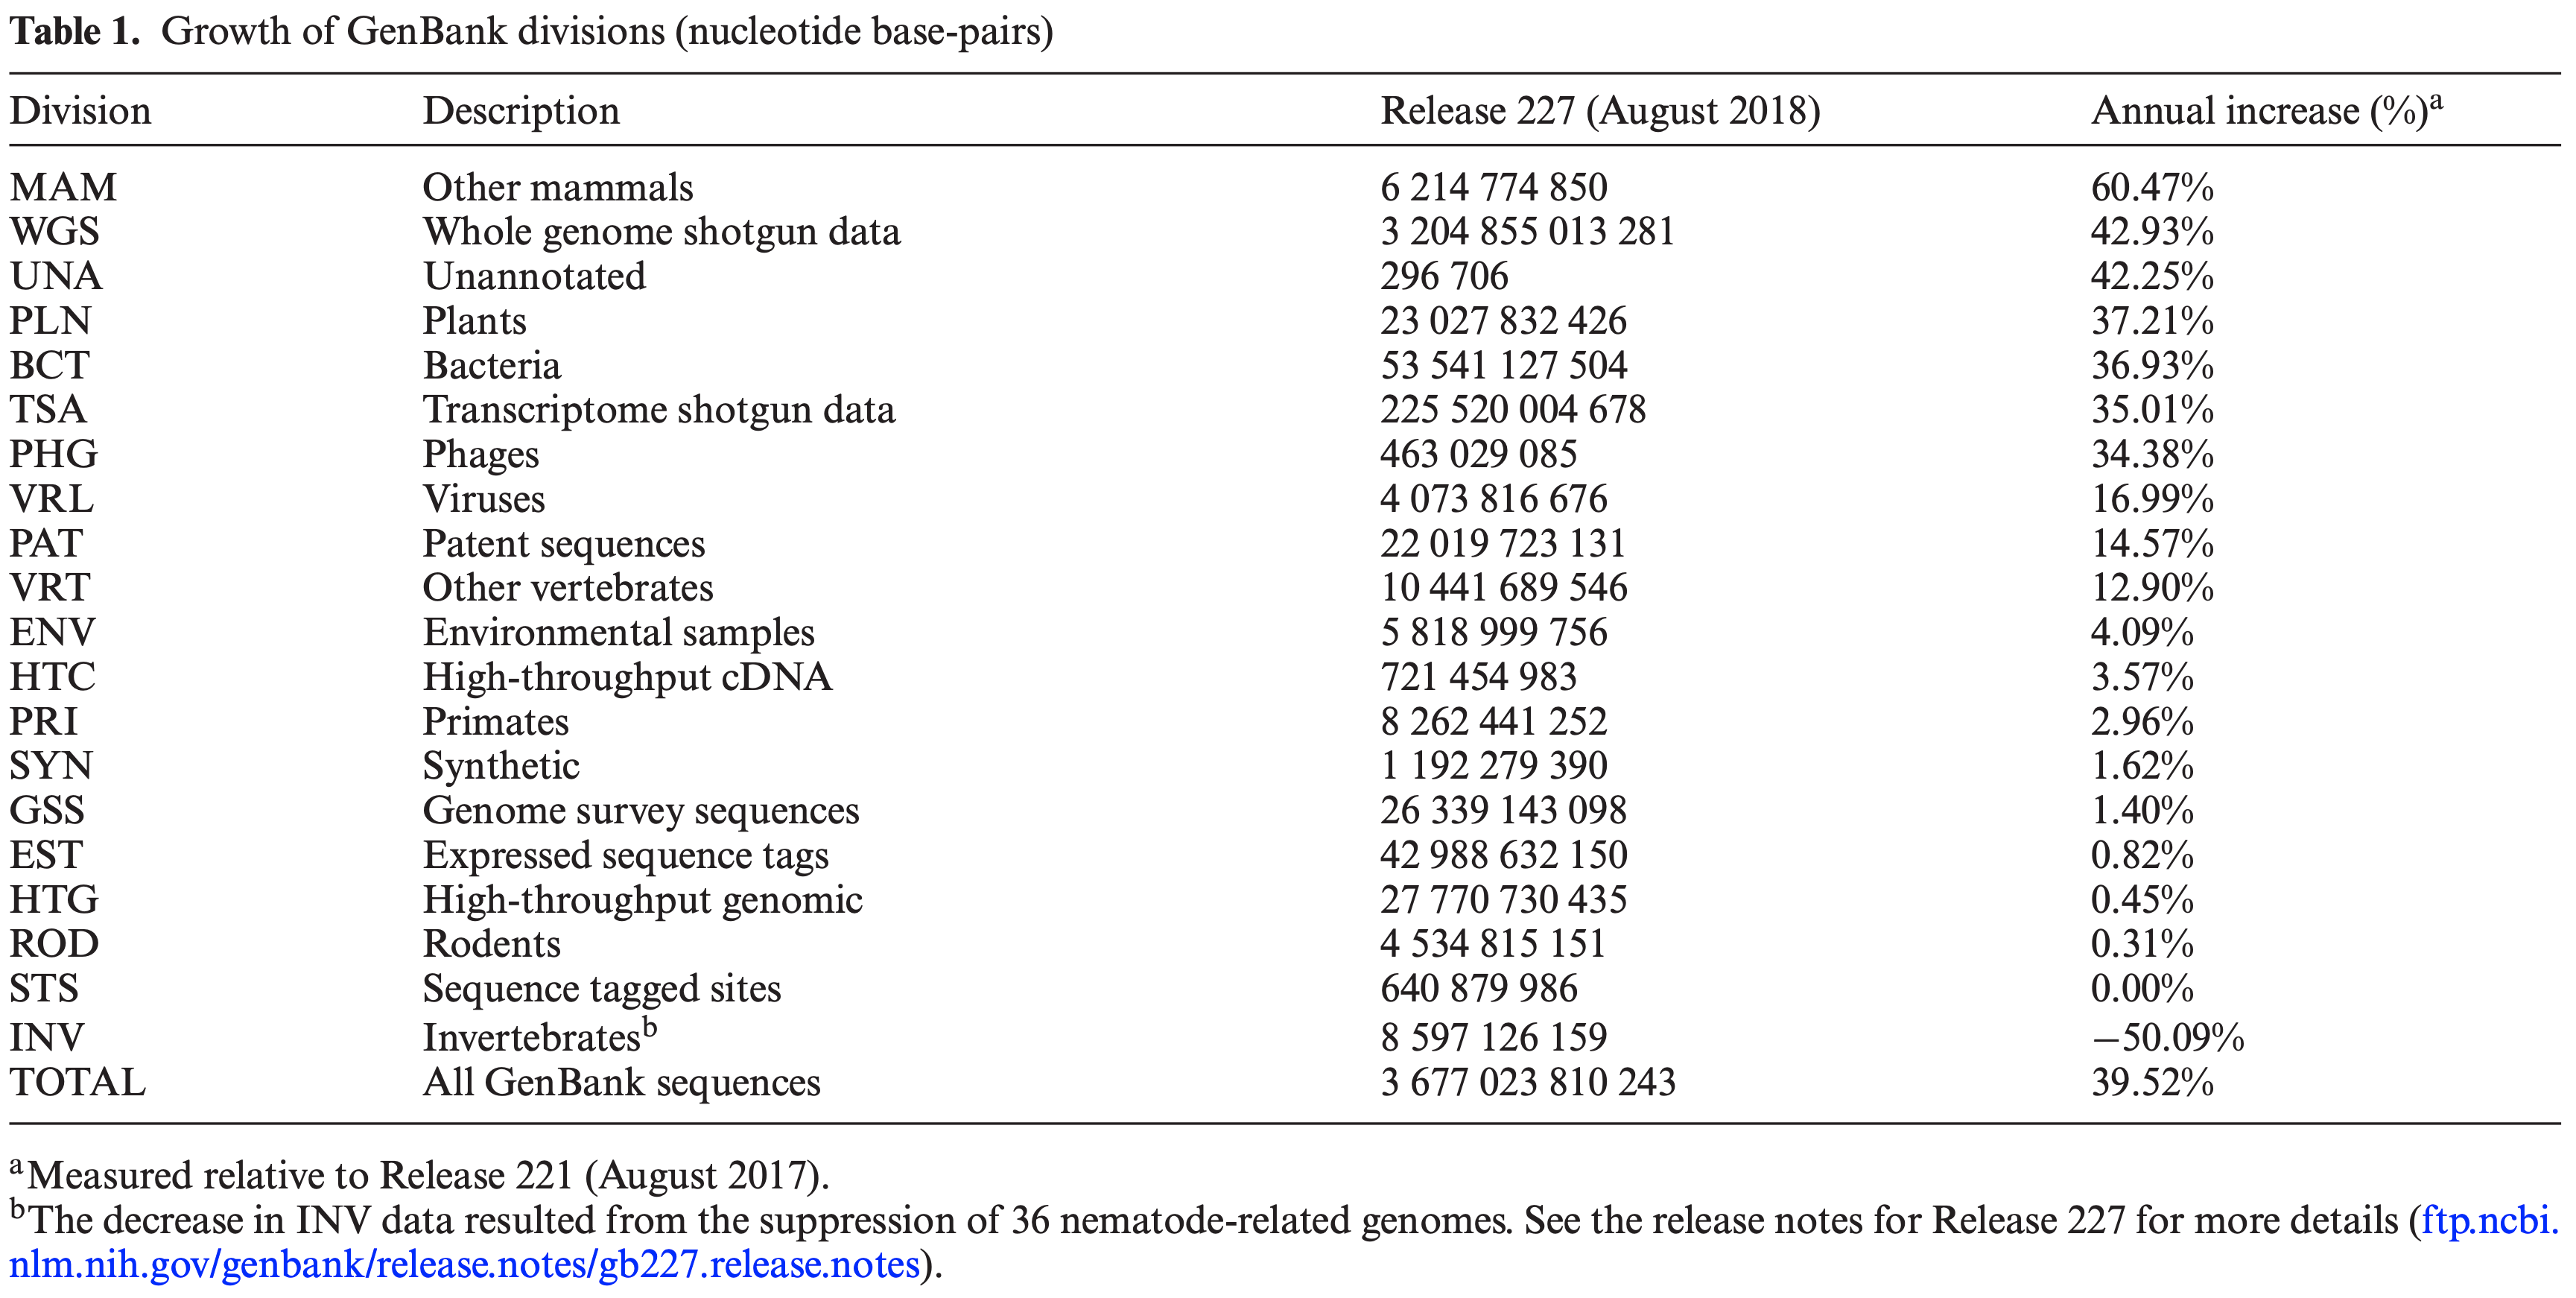
\includegraphics[width=9in]{figs/genbank-2019-table1}


\vfill
\end{slide}
%%%%%%%%%%%%%%%%%%%%%%%%%%%%%%%%%%%%%%%%%%%%%%%%%%%%%%%%%%%%%%%%%%%%%%
\begin{slide}
\begin{center}
\textbf{Manual NCBI GenBank indexing does not scale}

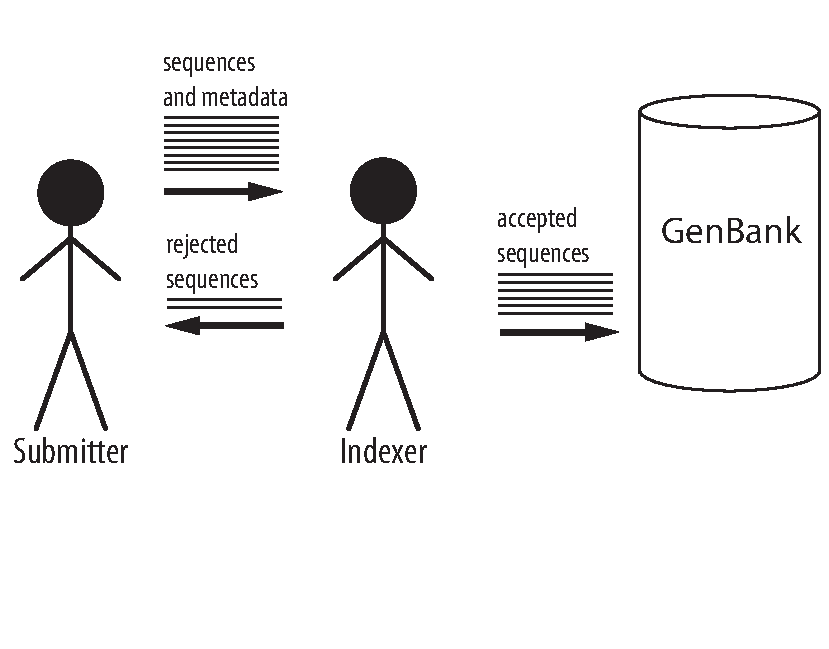
\includegraphics[width=7in]{figs/submission-schematic-1}

\vfill
\end{center}
\end{slide}
%%%%%%%%%%%%%%%%%%%%%%%%%%%%%%%%%%%%%%%%%%%%%%%%%%%%%%%%%%%%%%%%%%%%%%
\begin{slide}
\begin{center}
\textbf{Submissions can be grouped and analyzed based on sequence type}
\end{center}

\small
\begin{itemize}
\item Many submissions are of \emph{marker genes}, used to
  characterize environments (microbiome, soil), which are
  automatically analyzed by BLAST or specialized tools.
%\item Submissions with zero errors automatically enter database
%  (``foosh'')
%\item Submissions with errors can be corrected by submitter or are manually reviewed by an indexer
\end{itemize}

\medskip

\begin{center}
\begin{tabular}{lrr}
 marker gene/                    &  2018    & total \\
 sequence type                   &  \# seqs & \# seqs   \\ \hline
& & \\
%\textcolor{red}{16S rRNA}        & \textcolor{red}{333,121}  & \textcolor{red}{8,015,297} & \textcolor{red}{18,262,402} & \textcolor{red}{BLAST}\footnote{TLS submissions now processed with Ribosensor} \\
%16S rRNA                        & 333,121  & 8,015,297 & 18,262,402 & BLAST$^{*}$ \\
16S rRNA                        & 333,121  & 8,015,297 \\
& & \\                    
 COX1                            & 35,517  & 1,349,957  \\
& & \\                    
 23S rRNA                        & 74,287  &   275,014  \\
& & \\
 ITS1                            & 27,279  &   359,380  \\
& & \\                    
 ITS2                            & 24,144  &   184,515  \\
& & \\                    
 ITS1+ITS2                       & 26,734  &   445,721  \\
& & \\                    
 Influenza                       & 74,868  &   665,464  \\
\end{tabular}
\end{center}
\vfill
%\tiny \flushleft{$\dagger$ TLS: Targeted Locus Study, currently only 16S submissions with $>=$ 2500 seqs, handled by Anji Johnston}
%\tiny \flushleft{$\ddagger$ TLS submissions now processed with ribosensor}
\end{slide}
%%%%%%%%%%%%%%%%%%%%%%%%%%%%%%%%%%%%%%%%%%%%%%%%%%%%%%%%%%%%%%%%%%%%%%
\begin{slide}
\begin{center}
\textbf{NCBI GenBank Indexers use BLAST}

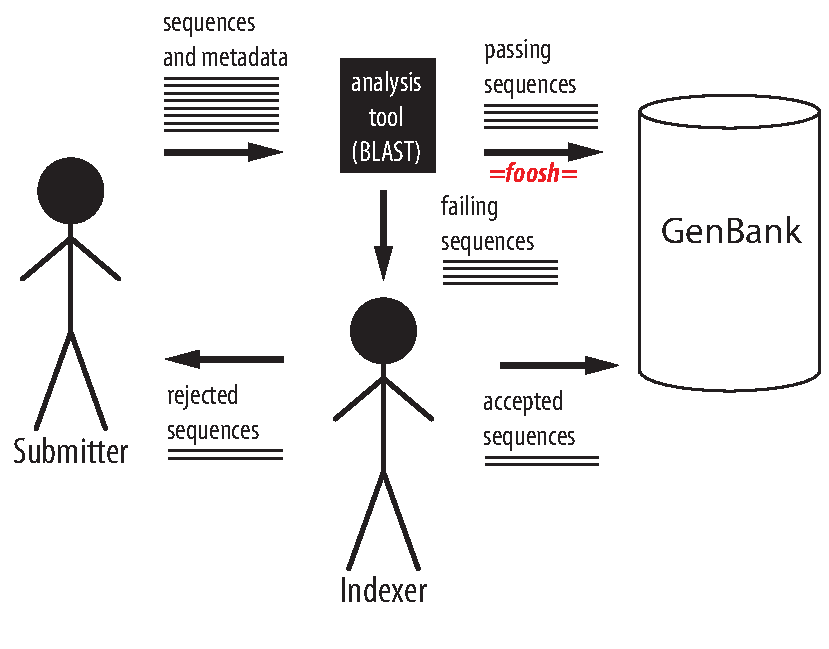
\includegraphics[width=7in]{figs/submission-schematic-2}

\small
\begin{itemize}
\item Foosh pipelines exist for 16S, 23S, ITS (BLAST-based) and
    Influenza (FLAN)
\end{itemize}

\vfill
\end{center}
\end{slide}
%%%%%%%%%%%%%%%%%%%%%%%%%%%%%%%%%%%%%%%%%%%%%%%%%%%%%%%%%%%%%%%%%%%%%%
\begin{slide}
\begin{center}
\textbf{NCBI GenBank Indexers use BLAST}

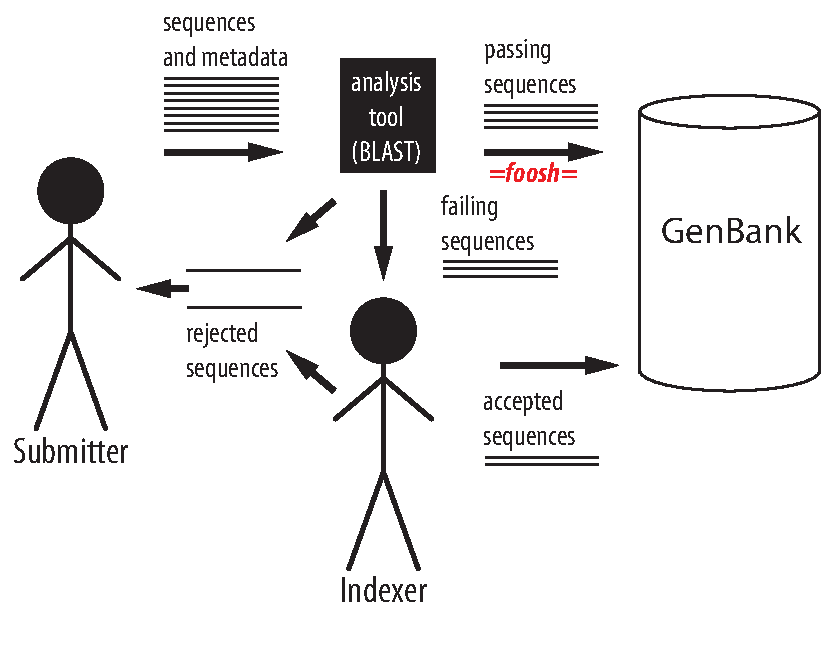
\includegraphics[width=7in]{figs/submission-schematic-3}

\small
\begin{itemize}
\item Foosh pipelines exist for 16S, 23S, ITS (BLAST-based) and
    Influenza (FLAN)
\end{itemize}

\vfill
\end{center}
\end{slide}
%%%%%%%%%%%%%%%%%%%%%%%%%%%%%%%%%%%%%%%%%%%%%%%%%%%%%%%%%%%%%%%%%%%%%%
\begin{slide}


\includegraphics[width=7in]{figs/blank-slide}
  
\vfill
\end{slide}
%%%%%%%%%%%%%%%%%%%%%%%%%%%%%%%%%%%%%%%%%%%%%%%%%%%%%%%%%%%%%%%%%%%%%%
\begin{slide}
\begin{center}

%\textbf{Viruses with highest number of sequences in INSDC\footnote{as of October, 2019.}}
\textbf{Viruses with highest number of sequences in GenBank\footnote{as of October, 2019.}}

\tiny
\begin{tabular}{lrl}
species                   &       \#seqs & family           \\ \hline
%                                                              % taxids
& & \\
HIV-1                     &      850,115 & \emph{Retroviridae}     \\ % 11676
& & \\
Influenza A virus         &      684,026 & \emph{Orthomyxoviridae} \\ % 11320
& & \\
Hepacivirus C             &      244,533 & \emph{Flaviviridae}     \\ % 11103
& & \\
Hepatitis B virus         &      114,306 & \emph{Hepadnaviridae}   \\ % 10407
& & \\
Influenza B virus         &      100,373 & \emph{Orthomyxoviridae} \\ % 11520
& & \\
Rotavirus A               &       73,375 & \emph{Reoviridae}       \\ % 28875
& & \\
SIV                       &       44,374 & \emph{Retroviridae}     \\ % 11723
& & \\
Norovirus (Norwalk virus) &       40,925 & \emph{Caliciviridae}    \\ % 11983
& & \\
Enterovirus A             &       31,478 & \emph{Picornaviridae}   \\ % 138948
& & \\
PRRSV                     &       29,081 & \emph{Arteriviridae}    \\ % 28344
& & \\
Dengue virus              &       28,564 & \emph{Flaviviridae}     \\ % 12637
& & \\
Human orthopneumovirus    &       24,384 & \emph{Pneumoviridae}    \\ % 11250 (RSV) 
& & \\
Enterovirus B             &       23,865 & \emph{Picornaviridae}   \\ % 138949
& & \\
Rabies lyssavirus         &       23,771 & \emph{Rhabdoviridae}    \\ % 11292
& & \\
West Nile virus           &       21,563 & \emph{Flaviviridae}     \\ % 11082
& & \\
Measles morbillivirus     &       17,233 & \emph{Paramyxoviridae}  \\ % 11234
\end{tabular}

\vfill

\end{center}
\end{slide}

%%%%%%%%%%%%%%%%%%%%%%%%%%%%%%%%%%%%%%%%%%%%%%%%%%%%%%%%%%%%%%%%%%%%%%
\begin{slide}
\begin{center}
\textbf{Viral sequences are not systematically or thoroughly annotated}
\end{center}
\medskip

\small
\begin{itemize}
\item Genome annotation of the Zika virus:
\end{itemize}  

\center{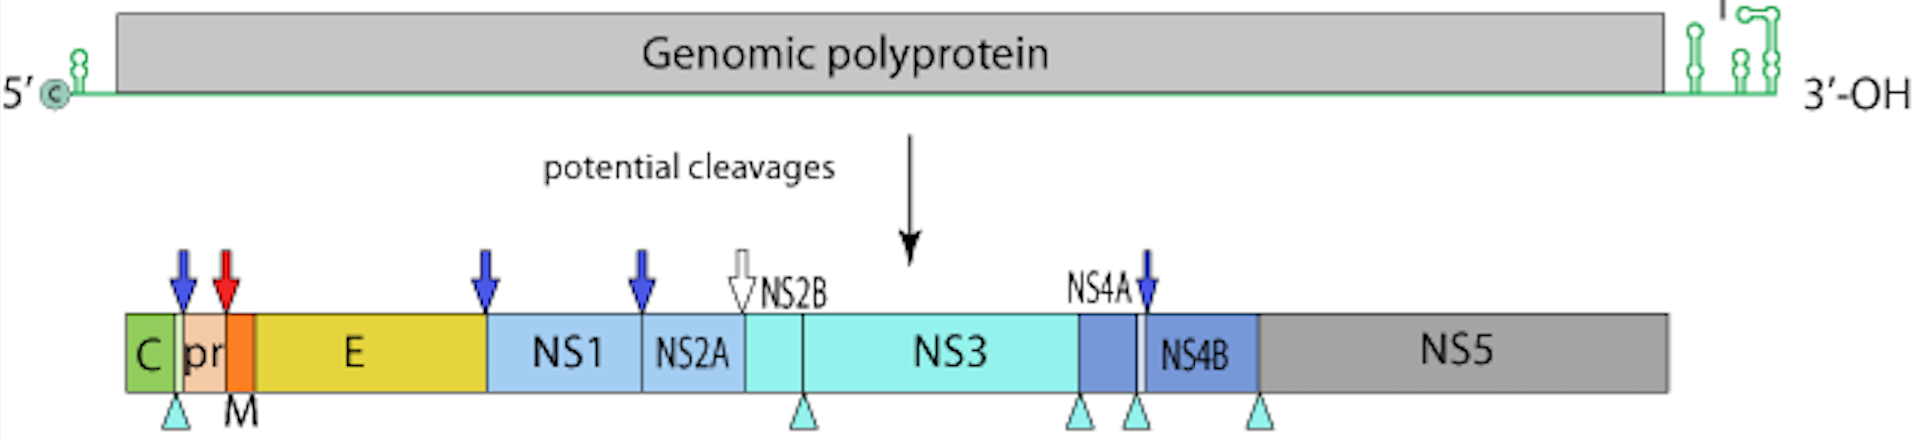
\includegraphics[width=8in]{figs/zika-genome-norna}}

\begin{itemize}
\item Zika's genome encodes a single polyprotein that is cleaved into 14 mature peptides.
\item Zika RefSeq annotation (NC\_012532) includes CDS and mature peptide annotation.
\end{itemize}

\vfill
\tiny \flushleft{figure from ViralZone, Hulo et al. NAR. 2011 Jan;39:D576-82}
\end{slide}
%%%%%%%%%%%%%%%%%%%%%%%%%%%%%%%%%%%%%%%%%%%%%%%%%%%%%%%%%%%%%%%%%%%%%%
\begin{slide}
\begin{center}
\textbf{Viral sequences are not systematically or thoroughly annotated}
\end{center}
\medskip

\small
\begin{itemize}
\item Genome annotation of the Zika virus:
\end{itemize}  

\center{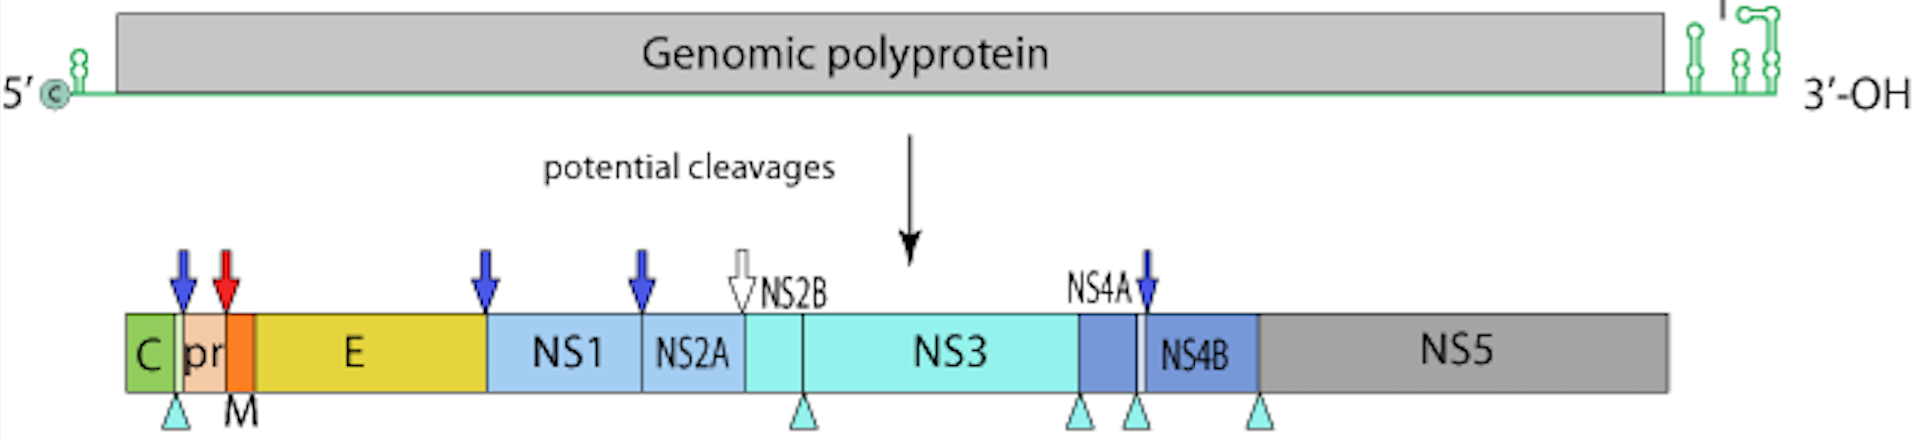
\includegraphics[width=8in]{figs/zika-genome-norna}}

\begin{itemize}
\item Zika's genome encodes a single polyprotein that is cleaved into 14 mature peptides.
\item Zika RefSeq annotation (NC\_012532) includes CDS and mature peptide annotation.
\item About 84\% of Zika virus sequences have CDS annotation.
\item Less than 25\% of Zika virus sequences have mature peptide annotation.
\item Less than 7\% of Dengue virus sequences have mature peptide annotation.
\item Less than 2\% of Norovirus sequences have mature peptide annotation.
\end{itemize}

\vfill
\tiny \flushleft{figure from ViralZone, Hulo et al. NAR. 2011 Jan;39:D576-82}
\end{slide}
%%%%%%%%%%%%%%%%%%%%%%%%%%%%%%%%%%%%%%%%%%%%%%%%%%%%%%%%%%%%%%%%%%%%
\begin{slide}
\begin{center}
\textbf{Viral sequences are not systematically or thoroughly annotated}
\end{center}
\medskip

\small
\begin{itemize}
\item Genome annotation of the Zika virus:
\end{itemize}  

\center{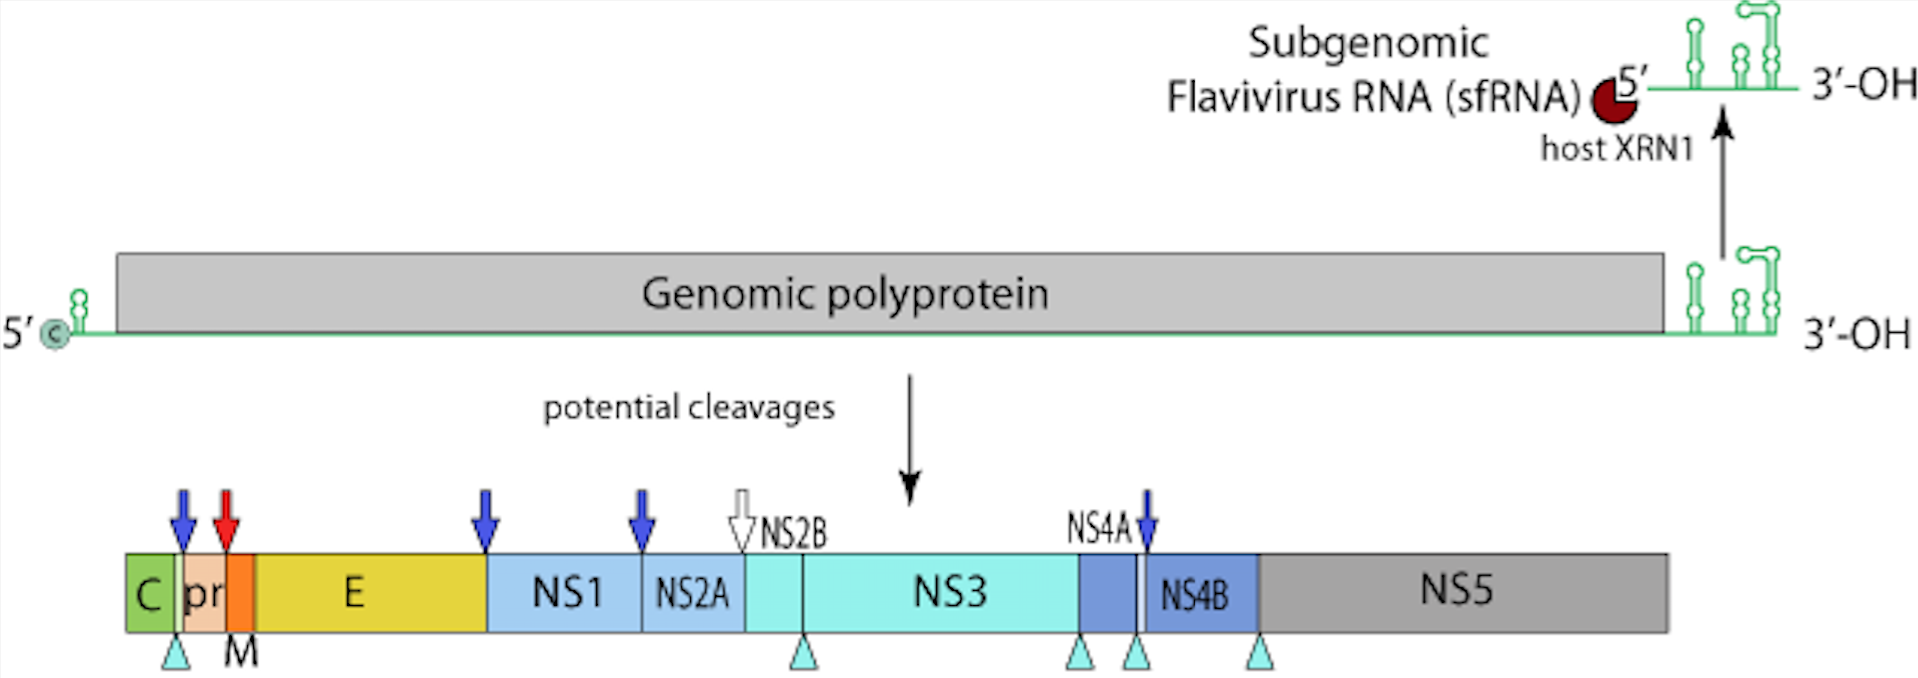
\includegraphics[width=8in]{figs/zika-genome-yesrna}}

\begin{itemize}
\item RNA structures in the 3' UTR halt host exonuclease leading to an
  accumulation of 300-500nt subgenomic flavivirus RNAs (sfRNAs) are
  related to pathogenicity.
\end{itemize}

\normalsize
\center{\textbf{\emph{These RNA structures are not annotated in the
      \\ Zika genome RefSeq (NC\_012532)}}}

\vfill
\tiny \flushleft{figure from ViralZone, Hulo et al. NAR. 2011 Jan;39:D576-82}
\end{slide}
%%%%%%%%%%%%%%%%%%%%%%%%%%%%%%%%%%%%%%%%%%%%%%%%%%%%%%%%%%%%%%%%%%%%%%
\begin{slide}
\begin{center}
\textbf{Viral sequences are not systematically or thoroughly annotated}
\end{center}

\small
\begin{itemize}
\item CDS are not always annotated
\item Mature peptides are rarely annotated
\item Rfam families are rarely to never annotated in viral genomes
  (roughly 200 families)
\end{itemize}

\normalsize
\center{\textbf{\emph{Systematic and complete annotation would \\ benefit viral
  researchers (facilitate comparative analyses)}}}

\vfill
\end{slide}
%%%%%%%%%%%%%%%%%%%%%%%%%%%%%%%%%%%%%%%%%%%%%%%%%%%%%%%%%%%%%%%%%%%%%%
\begin{slide}
\begin{center}
\textbf{Annotation and validation should be coupled}
\end{center}

\begin{center}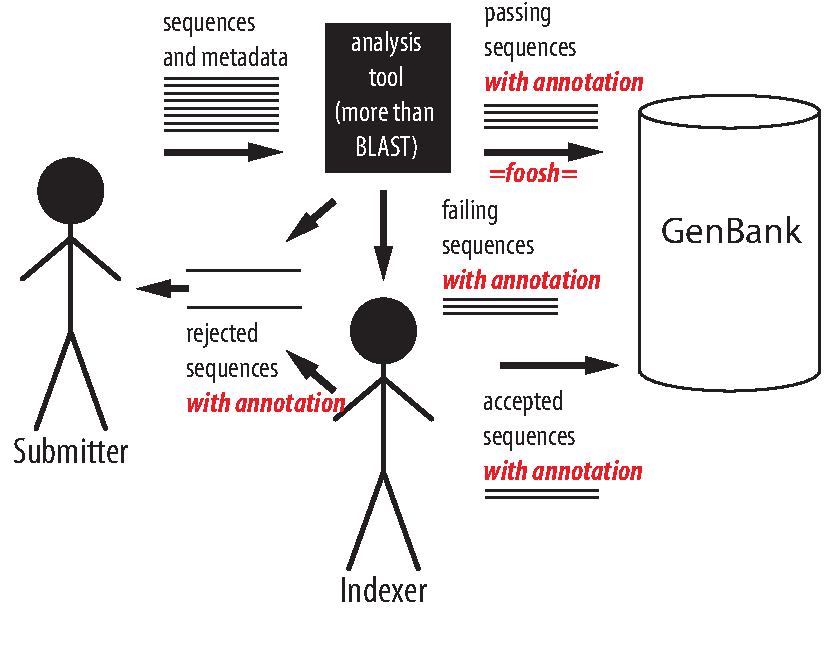
\includegraphics[width=7in]{figs/submission-schematic-4}\end{center}

\vfill
\end{slide}
%%%%%%%%%%%%%%%%%%%%%%%%%%%%%%%%%%%%%%%%%%%%%%%%%%%%%%%%%%%%%%%%%%%%%%
\begin{slide}
\begin{center}
\textbf{VADR (Viral Annotation DefineR) \\ uses RefSeqs to validate and
annotate viral sequences}

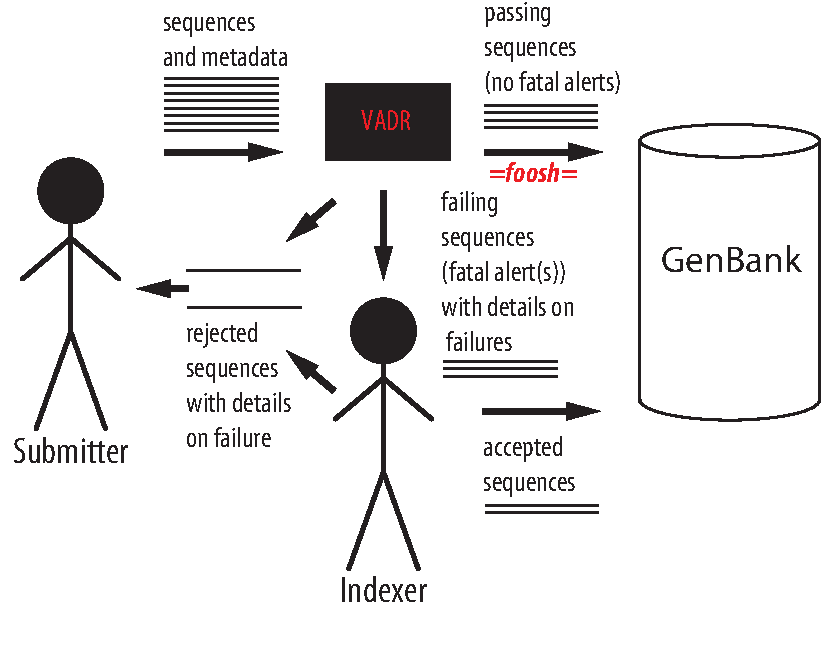
\includegraphics[width=7in]{figs/submission-schematic-5}
\end{center}

\small
\begin{itemize}
  \item Unexpected characteristics are reported as \emph{alerts}
    (e.g. early stop codon)
  \item Some alerts are \emph{fatal} and cause sequences to \emph{fail}
\end{itemize}

%\small
%\begin{itemize}
%\item Build a model (covariance model) from a RefSeq (or alignment) using \texttt{v-build.pl}
%\begin{itemize}
%  \item includes boundaries of CDS, mat\_peptide, ncRNA and other features
%\end{itemize}

%\item Incoming sequences are compared against a library of models to find
%  the best-matching model which is used to annotate the sequence using
%  \texttt{v-annotate.pl}.

\vfill
\end{slide}
%%%%%%%%%%%%%%%%%%%%%%%%%%%%%%%%%%%%%%%%%%%%%%%%%%%%%%%%%%%%%%%%%%%%%%
\begin{slide}
\begin{center}

\textbf{Norovirus and Dengue virus chosen as first viruses for VADR testing}

\tiny
\begin{tabular}{lrl}
species                   &       \#seqs & family           \\ \hline
%                                                              % taxids
& & \\
HIV-1                     &      850,115 & \emph{Retroviridae}     \\ % 11676
& & \\
Influenza A virus         &      684,026 & \emph{Orthomyxoviridae} \\ % 11320
& & \\
Hepacivirus C             &      244,533 & \emph{Flaviviridae}     \\ % 11103
& & \\
Hepatitis B virus         &      114,306 & \emph{Hepadnaviridae}   \\ % 10407
& & \\
Influenza B virus         &      100,373 & \emph{Orthomyxoviridae} \\ % 11520
& & \\
Rotavirus A               &       73,375 & \emph{Reoviridae}       \\ % 28875
& & \\
SIV                       &       44,374 & \emph{Retroviridae}     \\ % 11723
& & \\
\textcolor{red}{Norovirus (Norwalk virus)} &       \textcolor{red}{40,925} & \textcolor{red}{\emph{Caliciviridae}}    \\ % 11983
& & \\
Enterovirus A             &       31,478 & \emph{Picornaviridae}   \\ % 138948
& & \\
PRRSV                     &       29,081 & \emph{Arteriviridae}    \\ % 28344
& & \\
%Dengue virus              &       28,564 & \emph{Flaviviridae}     \\ % 12637
\textcolor{red}{Dengue virus}              &       \textcolor{red}{28,564} & \textcolor{red}{\emph{Flaviviridae}}     \\ % 12637
& & \\
Human orthopneumovirus    &       24,384 & \emph{Pneumoviridae}    \\ % 11250 (RSV) 
& & \\
Enterovirus B             &       23,865 & \emph{Picornaviridae}   \\ % 138949
& & \\
Rabies lyssavirus         &       23,771 & \emph{Rhabdoviridae}    \\ % 11292
& & \\
West Nile virus           &       21,563 & \emph{Flaviviridae}     \\ % 11082
& & \\
Measles morbillivirus     &       17,233 & \emph{Paramyxoviridae}  \\ % 11234
\end{tabular}

\vfill

\end{center}
\end{slide}

%%%%%%%%%%%%%%%%%%%%%%%%%%%%%%%%%%%%%%%%%%%%%%%%%%%%%%%%%%%%%%%%%%%%%%
\begin{slide}
\begin{center}
%\textbf{VADR build step (\texttt{v-build.pl}) builds a homology model
\textbf{VADR build step (\texttt{v-build}) builds a homology model
  \\ (covariance model (CM)) of a RefSeq and stores feature information}

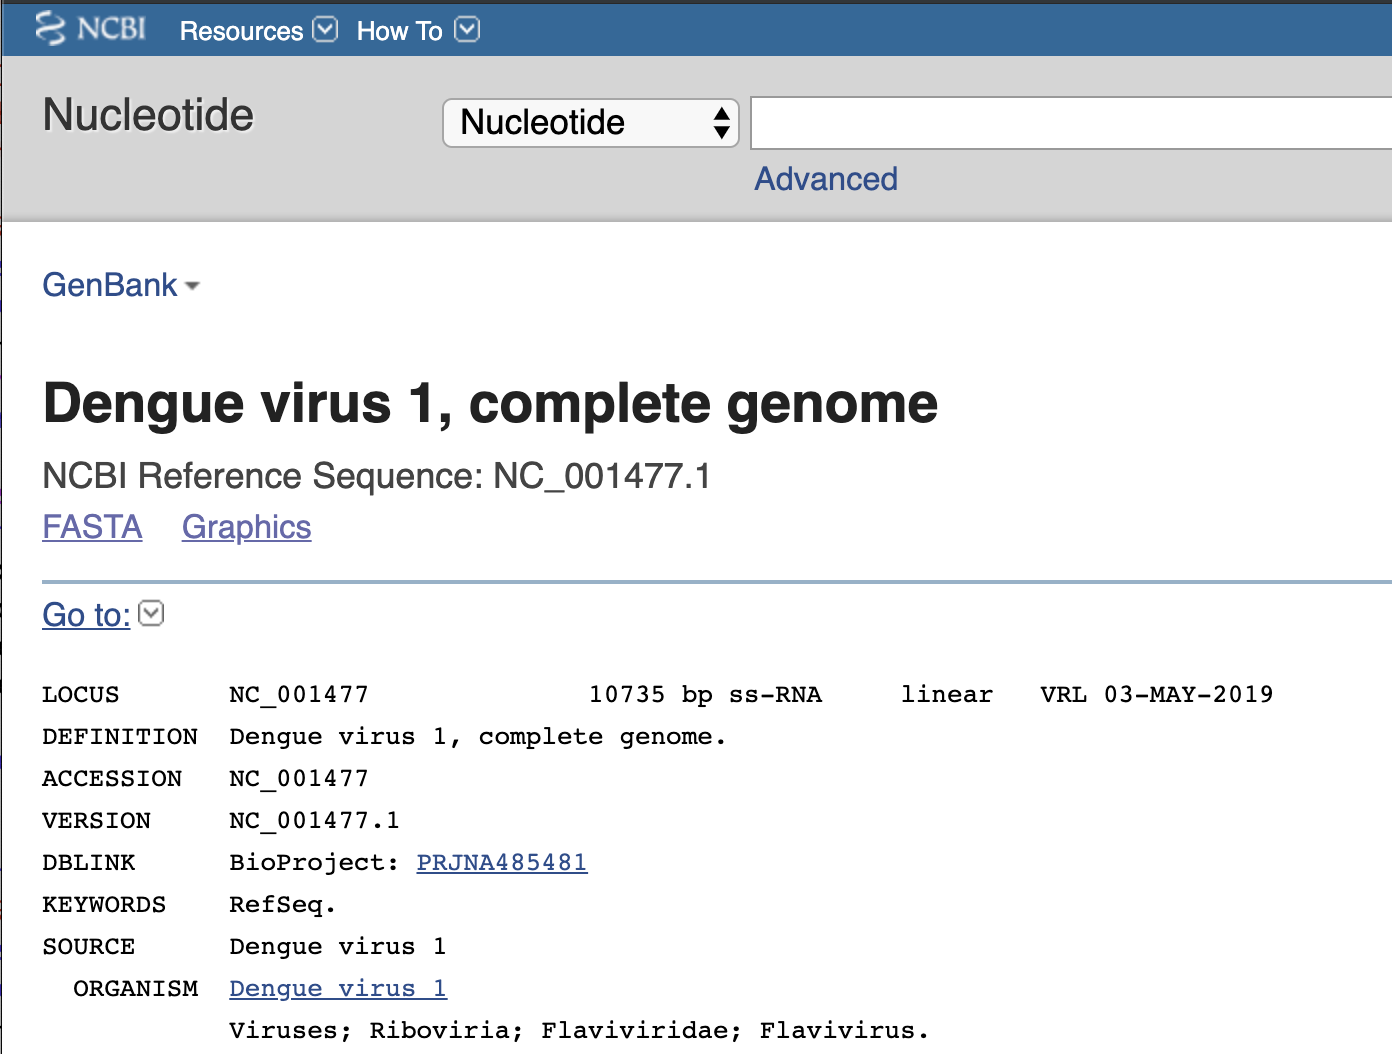
\includegraphics[width=6in]{figs/ss-001477-top}

\end{center}
\vfill
\end{slide}
%%%%%%%%%%%%%%%%%%%%%%%%%%%%%%%%%%%%%%%%%%%%%%%%%%%%%%%%%%%%%%%%%%%%%%
\begin{slide}
\begin{center}
%\textbf{VADR build step (\texttt{v-build.pl}) builds a homology model
\textbf{VADR build step (\texttt{v-build}) builds a homology model
  \\ (covariance model (CM)) of a RefSeq and stores feature information}

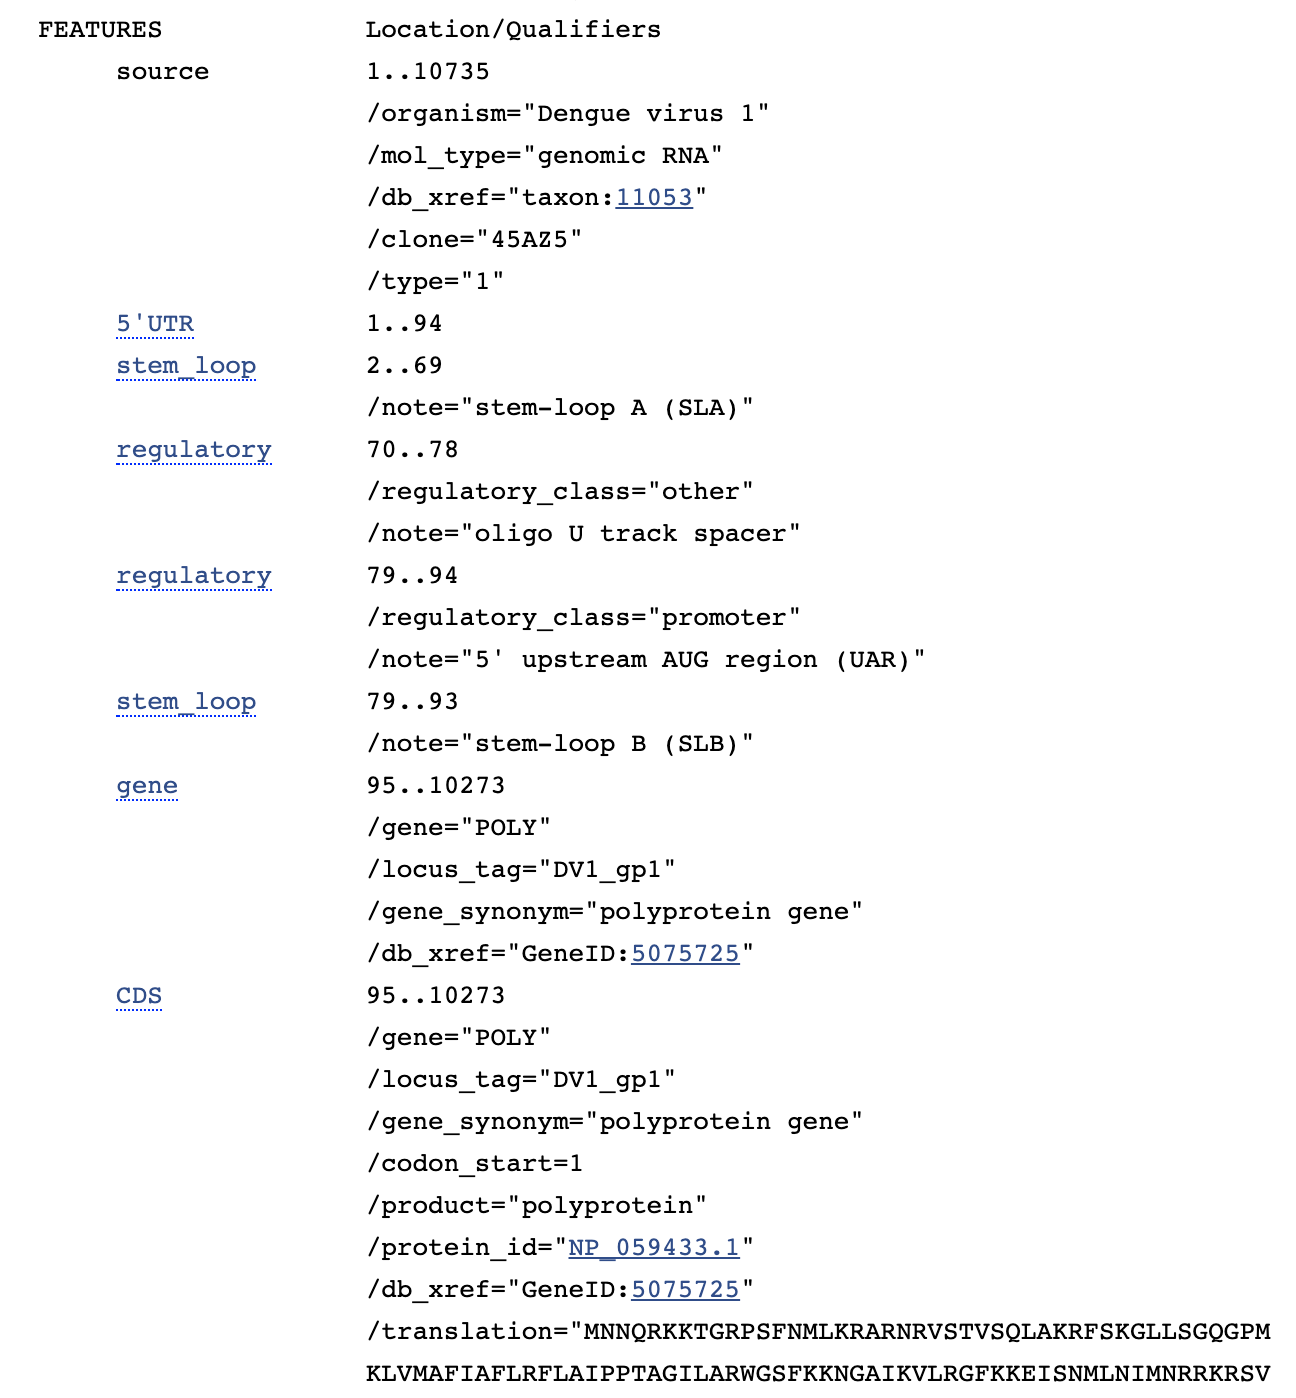
\includegraphics[width=6in]{figs/ss-001477-mid}

\end{center}
\vfill
\end{slide}
%%%%%%%%%%%%%%%%%%%%%%%%%%%%%%%%%%%%%%%%%%%%%%%%%%%%%%%%%%%%%%%%%%%%%%
\begin{slide}
\begin{center}
%\textbf{VADR build step (\texttt{v-build.pl}) builds a homology model
\textbf{VADR build step (\texttt{v-build}) builds a homology model
  \\ (covariance model (CM)) of a RefSeq and stores feature information}

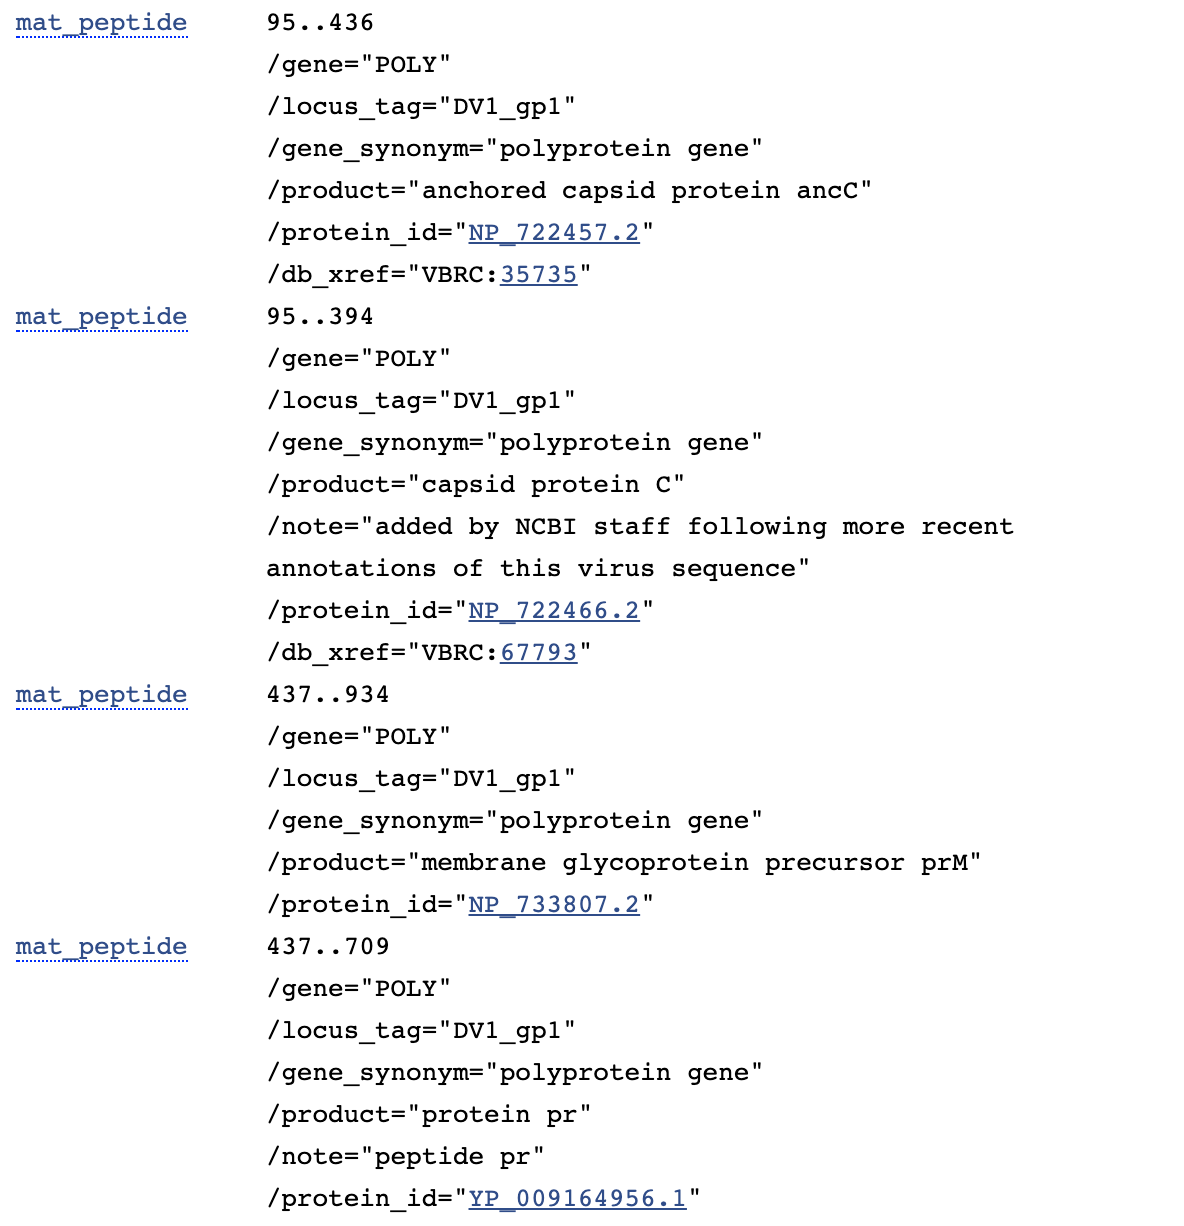
\includegraphics[width=6in]{figs/ss-001477-bot}

\end{center}
\vfill
\end{slide}
%%%%%%%%%%%%%%%%%%%%%%%%%%%%%%%%%%%%%%%%%%%%%%%%%%%%%%%%%%%%%%%%%%%%%%
\begin{slide}
\begin{center}
%\textbf{VADR build step (\texttt{v-build.pl}) builds a homology model
\textbf{VADR build step (\texttt{v-build}) builds a homology model
  \\ (covariance model (CM)) of a RefSeq and stores feature information}

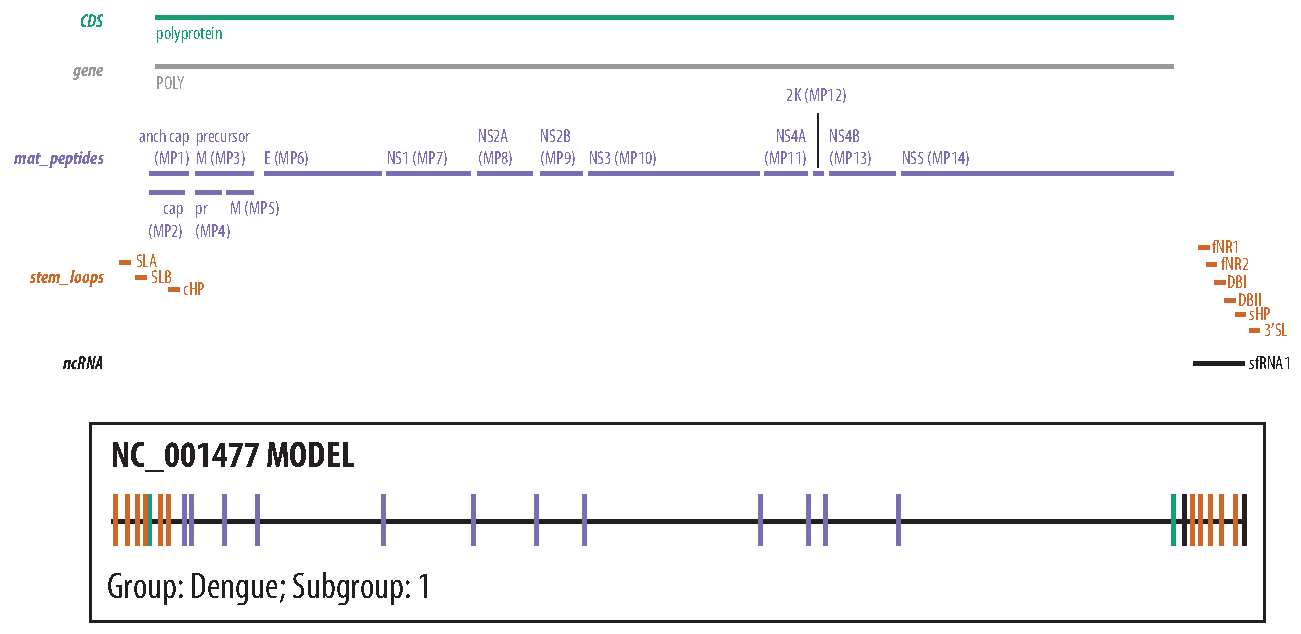
\includegraphics[width=10.5in]{figs/dengue-features}

\end{center}
\vfill
\end{slide}
%%%%%%%%%%%%%%%%%%%%%%%%%%%%%%%%%%%%%%%%%%%%%%%%%%%%%%%%%%%%%%%%%%%%%%
\begin{comment}
%%%%%%%%%%%%%%%%%%%%%%%%%%%%%%%%%%%%%%%%%%%%%%%%%%%%%%%%%%%%%%%%%%%%%%
\begin{slide}
\begin{center}
%\textbf{VADR build step (\texttt{v-build.pl}) builds a homology model
\textbf{VADR build step (\texttt{v-build}) builds a homology model
  \\ (covariance model (CM)) of a RefSeq and stores feature information}

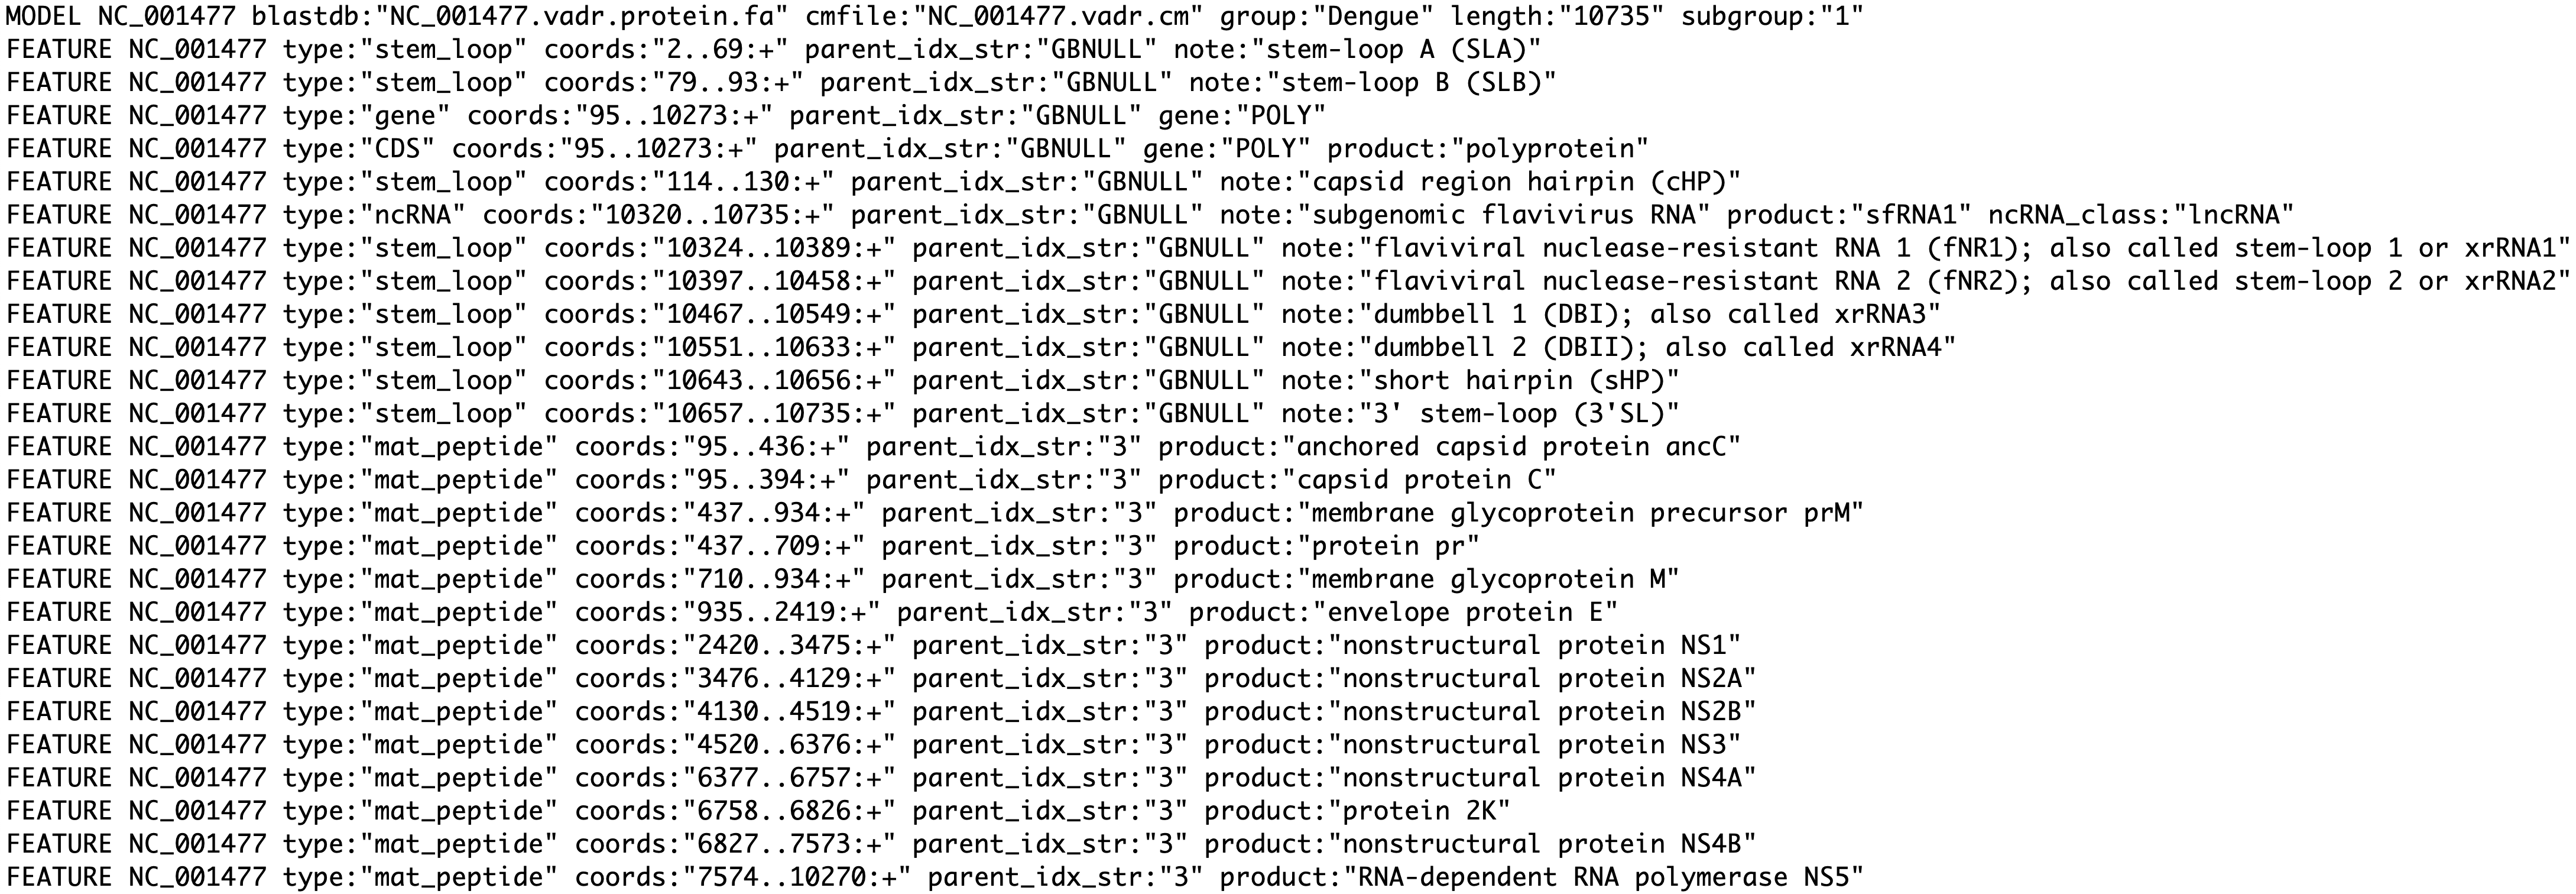
\includegraphics[width=10.5in]{figs/ss-001477-minfo}

\end{center}
\vfill
\end{slide}
%%%%%%%%%%%%%%%%%%%%%%%%%%%%%%%%%%%%%%%%%%%%%%%%%%%%%%%%%%%%%%%%%%%%%%
\end{comment}
%%%%%%%%%%%%%%%%%%%%%%%%%%%%%%%%%%%%%%%%%%%%%%%%%%%%%%%%%%%%%%%%%%%%%%
\begin{slide}
\begin{center}

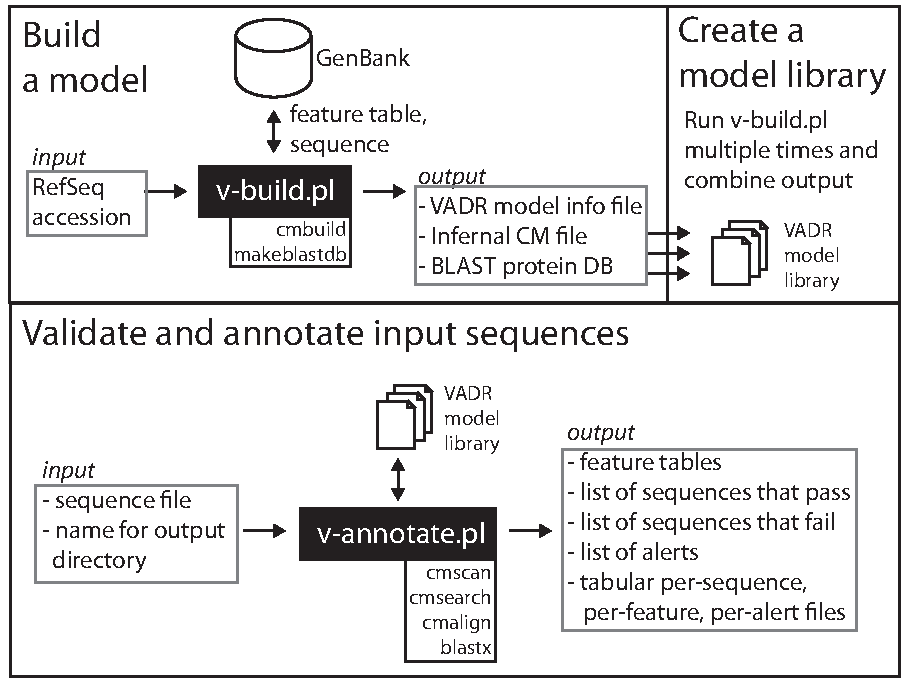
\includegraphics[width=10in]{figs/vadr}

\end{center}
\vfill
\end{slide}
%%%%%%%%%%%%%%%%%%%%%%%%%%%%%%%%%%%%%%%%%%%%%%%%%%%%%%%%%%%%%%%%%%%%%%
\begin{slide}
\begin{center}
\normalsize
\textbf{VADR 1.0 model library}

% /panfs/pan1/infernal/notebook/19_0520_vadr_build_from_ft/00LOG.txt
% 41 of the '197' models are Caliciviridae
% 156 of the '197' models are Flaviviridae
% But we purposefully omitted 3 new Norovirus from Flaviviridae, so
% it's 41 and 153.

\small
\begin{itemize}
\item 38 \emph{Caliciviridae} models:
  \begin{itemize}
  \item \textcolor{red}{9 Norovirus models}
  \item 7 Sapovirus models
  \item 4 Vesivirus models
    %  \item 18 other Caliciviruses
  \end{itemize}
\item 156 \emph{Flaviviridae} models:
  \begin{itemize}
  \item 10 Pegivirus models
%  \item \textcolor{red}{8 HCV models}
  \item 8 HCV models
  \item 7 Pestivirus models
  \item \textcolor{red}{4 Dengue virus models}
  \item 2 West Nile virus models
  \item 2 Zika virus models
  \end{itemize}
\end{itemize}

\end{center}

\vfill
\end{slide}
%%%%%%%%%%%%%%%%%%%%%%%%%%%%%%%%%%%%%%%%%%%%%%%%%%%%%%%%%%%%%%%%%%%%%%
\begin{slide}
\begin{center}
%\textbf{\texttt{v-annotate.pl} annotates each sequence using its
\textbf{\texttt{v-annotate} annotates each sequence using its
  best-matching model}

\begin{itemize}
\item For each sequence $S$:
\small
\begin{enumerate}
\item \textbf{Classification}: compare $S$ to all models to find best matching model $M$
\item \textbf{Coverage determination}: search $M$ against $S$ to find 'hits'
\item \textbf{Alignment}: align $S$ to $M$ and map features from $M$ to $S$
\item \textbf{Protein validation}: compare predicted CDS in $S$ to proteins
  from $M$ using BLASTX
\end{enumerate}
\end{itemize}

\emph{Different types of alerts are identified and reported at each stage}

\end{center}

\vfill
\end{slide}
%%%%%%%%%%%%%%%%%%%%%%%%%%%%%%%%%%%%%%%%%%%%%%%%%%%%%%%%%%%%%%%%%%%%%%
\begin{slide}
\begin{center}

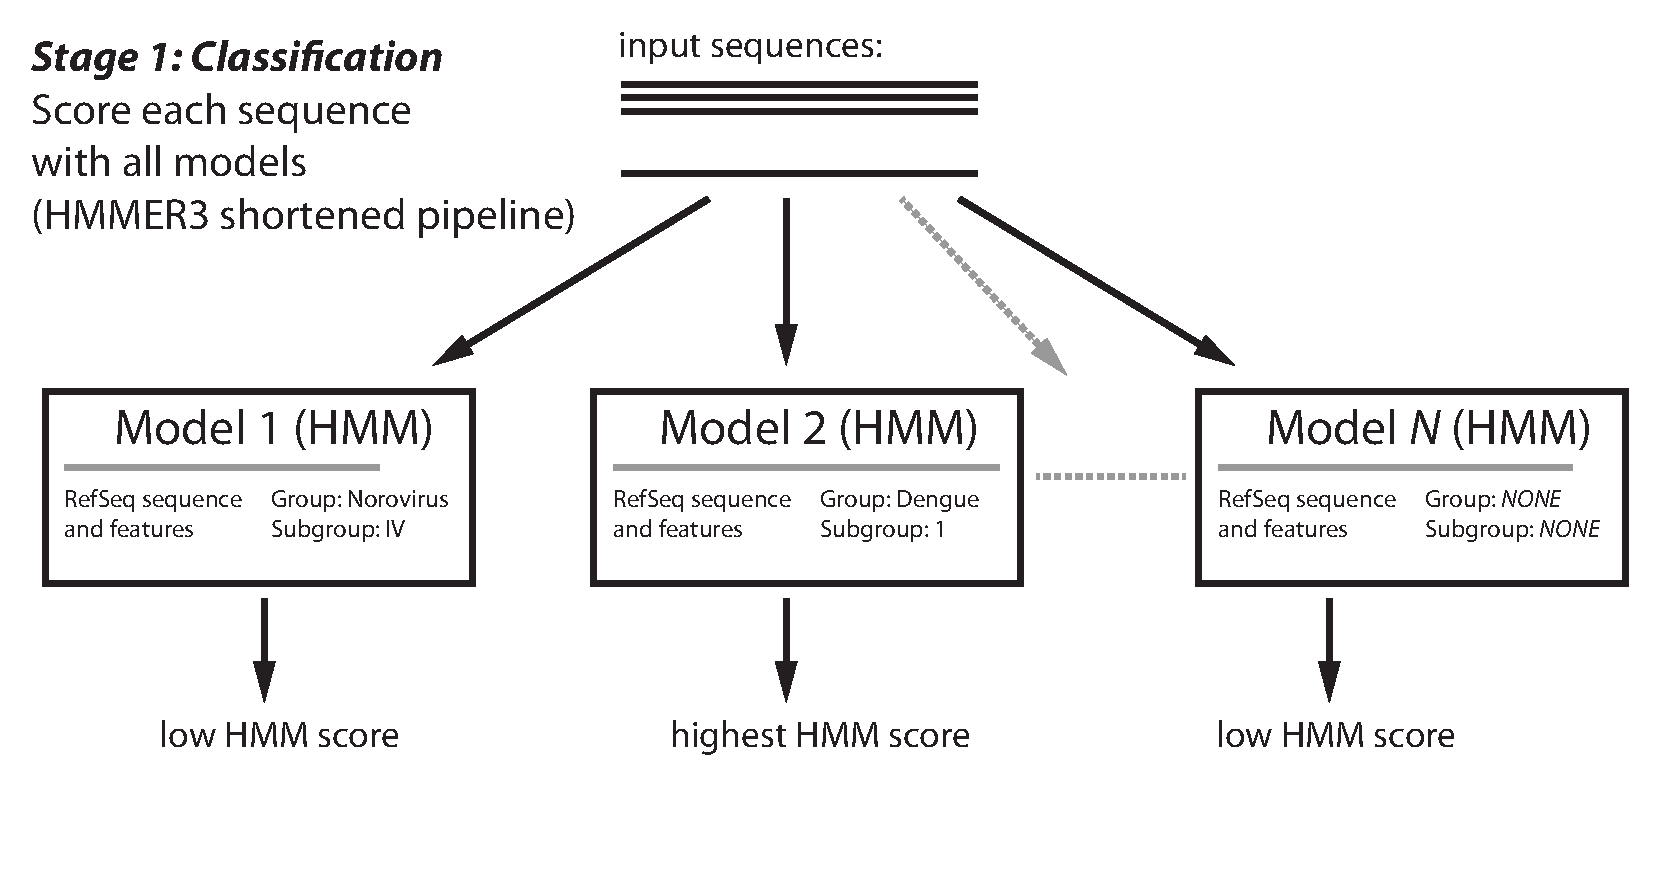
\includegraphics[width=9.5in]{figs/v-annotate-stage1-1}

\end{center}
\vfill
\end{slide}
%%%%%%%%%%%%%%%%%%%%%%%%%%%%%%%%%%%%%%%%%%%%%%%%%%%%%%%%%%%%%%%%%%%%%%
\begin{slide}
\begin{center}

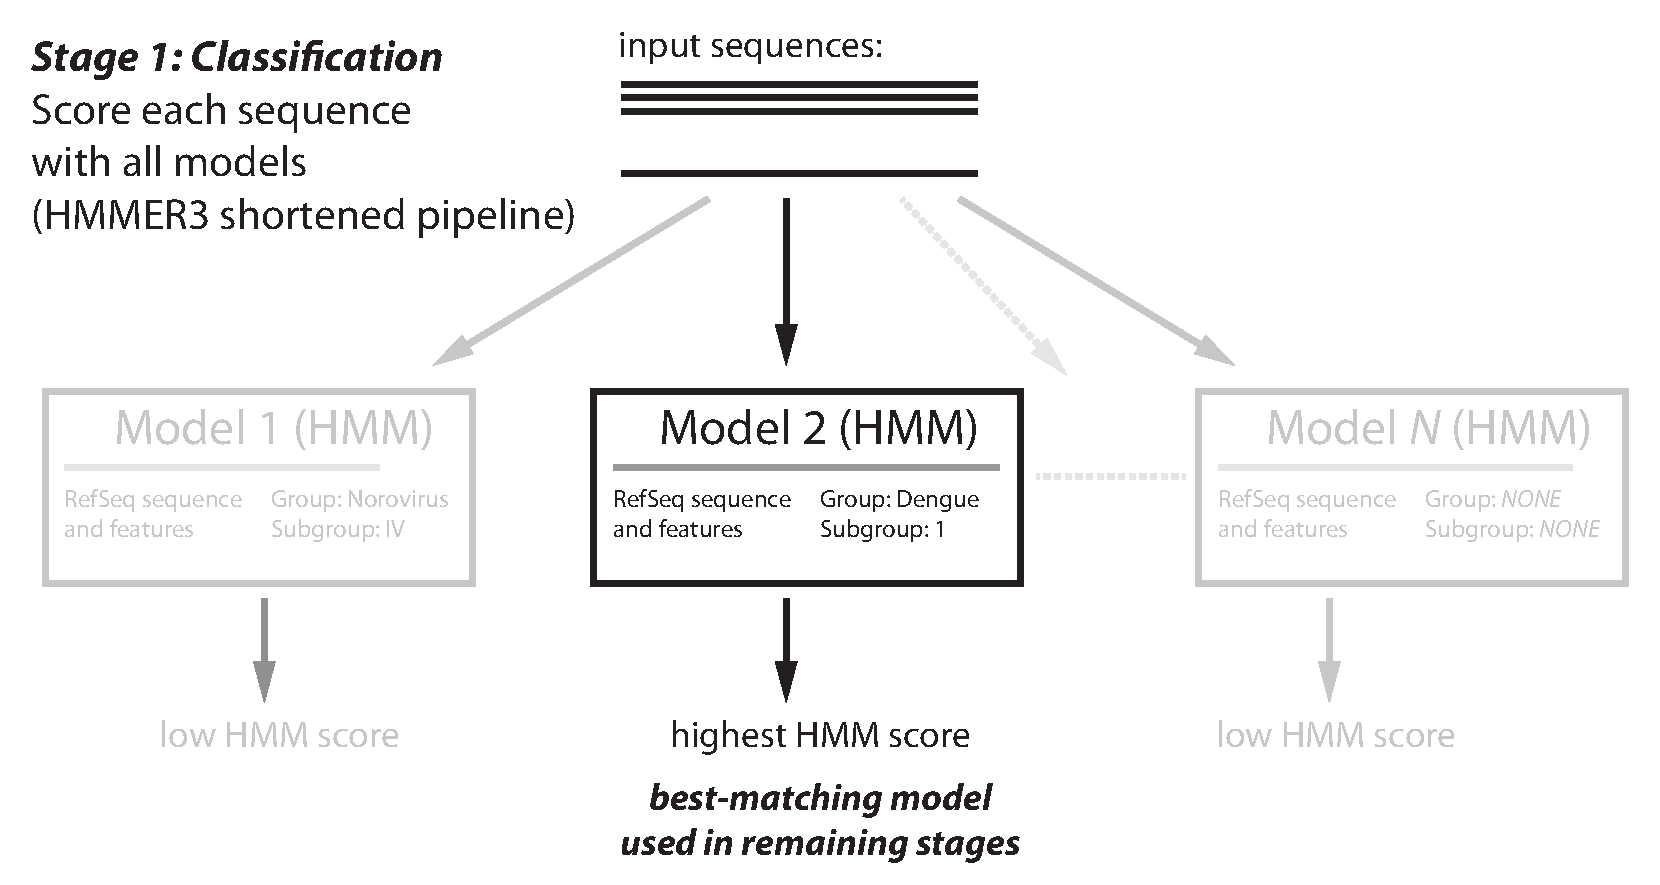
\includegraphics[width=9.5in]{figs/v-annotate-stage1-2}

\end{center}
\vfill
\end{slide}
%%%%%%%%%%%%%%%%%%%%%%%%%%%%%%%%%%%%%%%%%%%%%%%%%%%%%%%%%%%%%%%%%%%%%%
\begin{slide}
\begin{center}

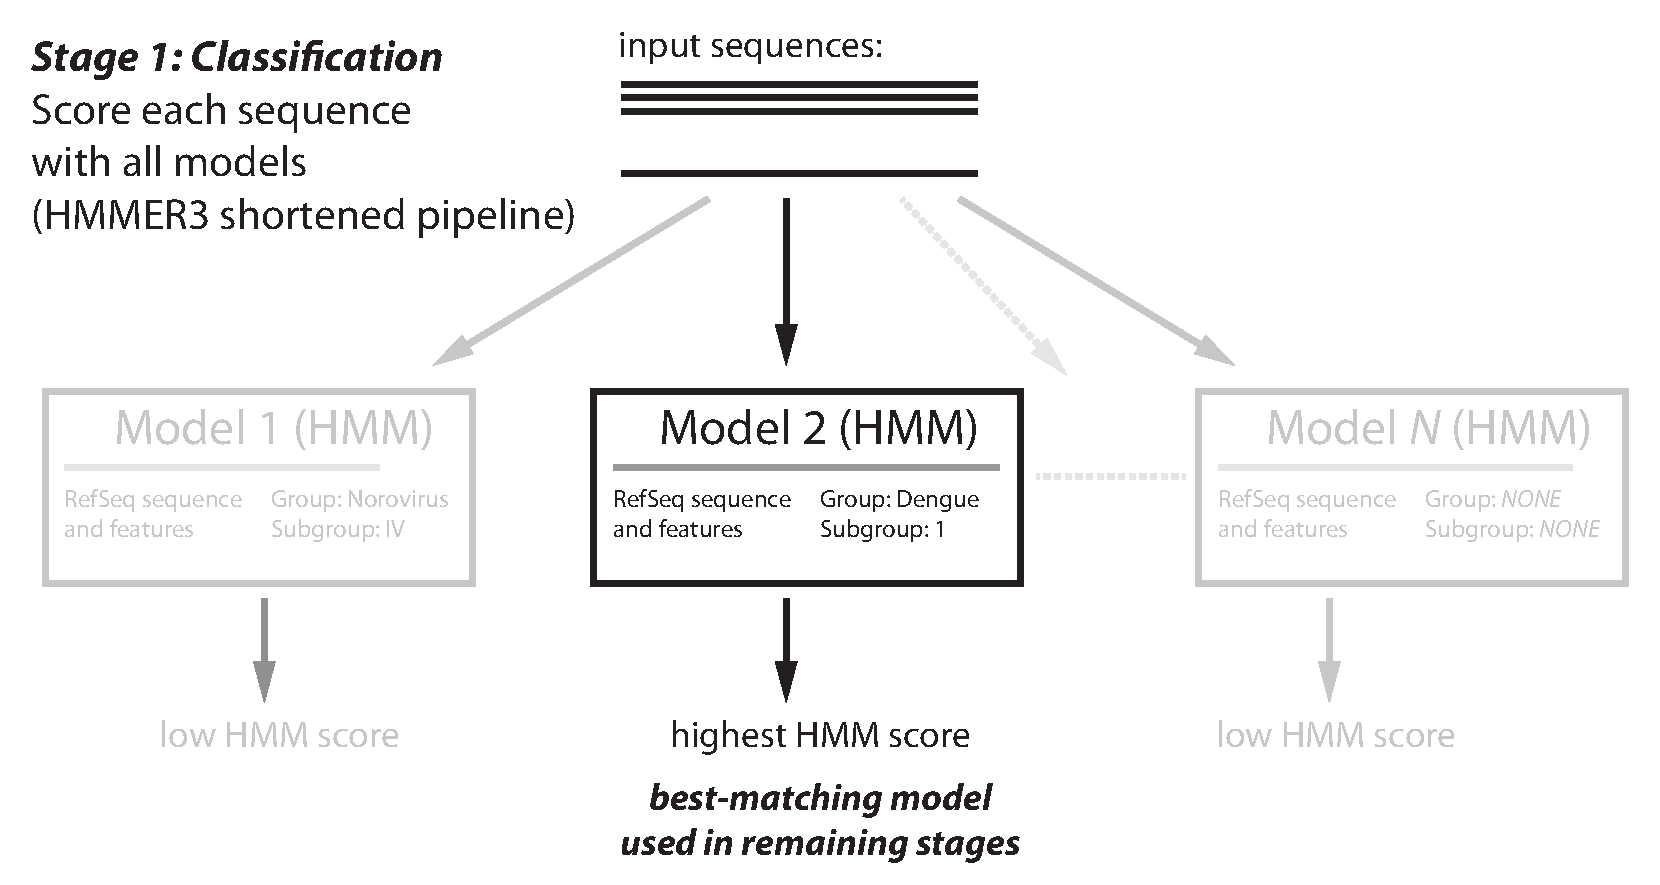
\includegraphics[width=9.5in]{figs/v-annotate-stage1-2}

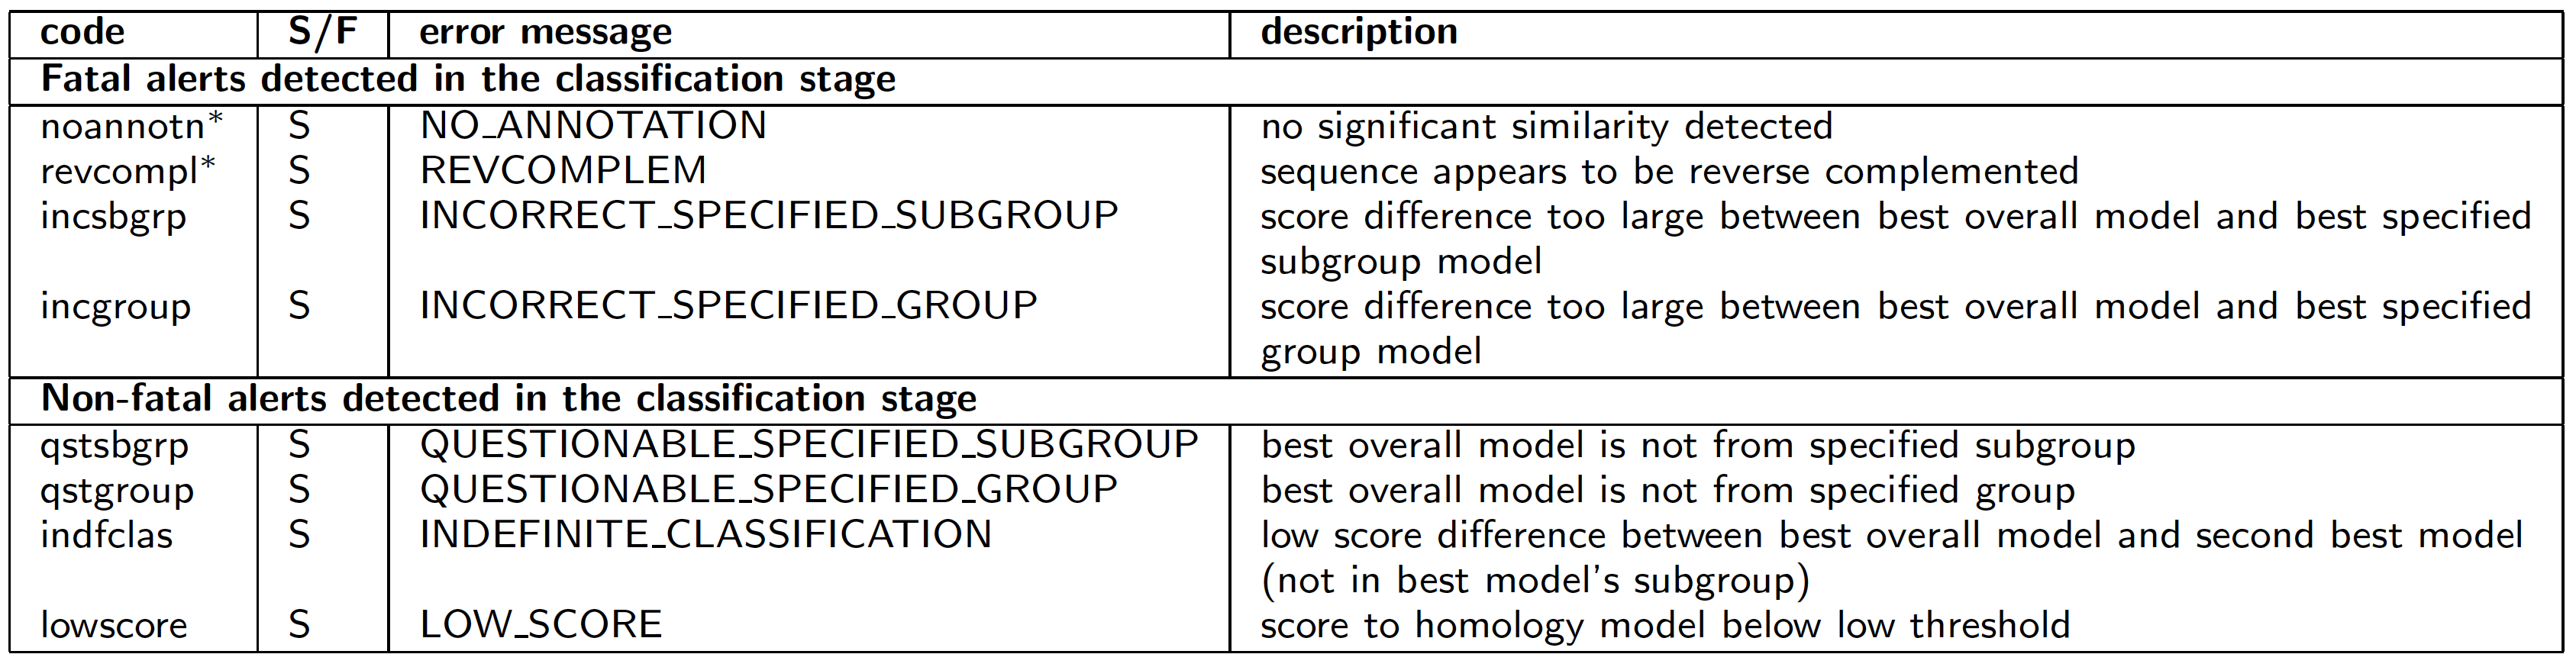
\includegraphics[width=10.5in]{figs/ss-class-alert-list}

\end{center}
\vfill
\end{slide}
%%%%%%%%%%%%%%%%%%%%%%%%%%%%%%%%%%%%%%%%%%%%%%%%%%%%%%%%%%%%%%%%%%%%%%
\begin{slide}
\begin{center}

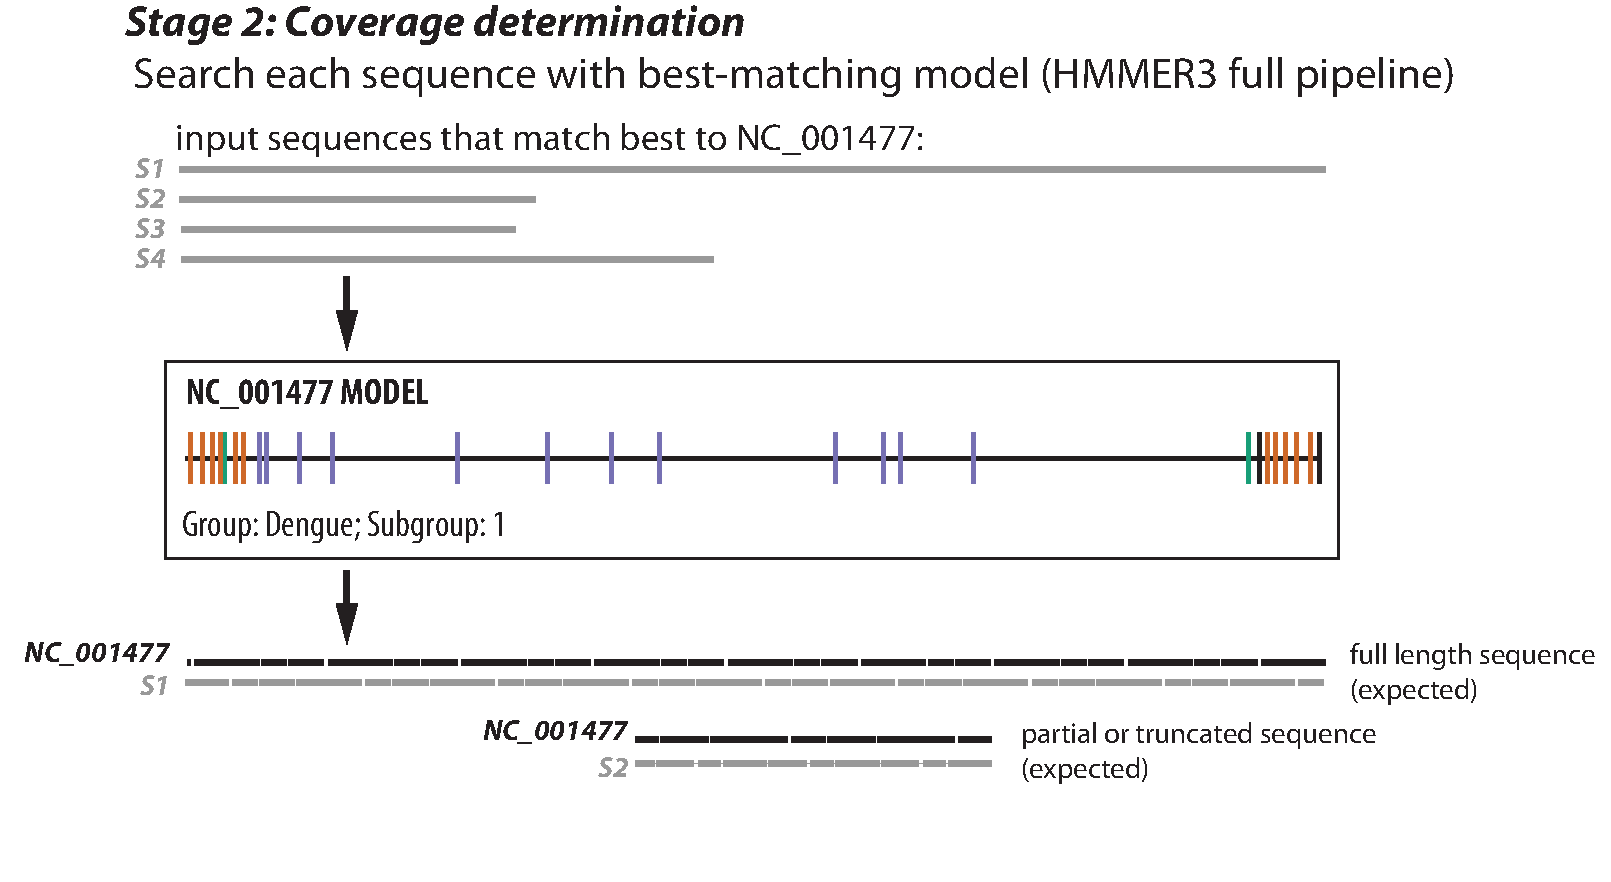
\includegraphics[width=10.5in]{figs/v-annotate-stage2-1}

\end{center}
\vfill
\end{slide}
%%%%%%%%%%%%%%%%%%%%%%%%%%%%%%%%%%%%%%%%%%%%%%%%%%%%%%%%%%%%%%%%%%%%%%
\begin{slide}
\begin{center}

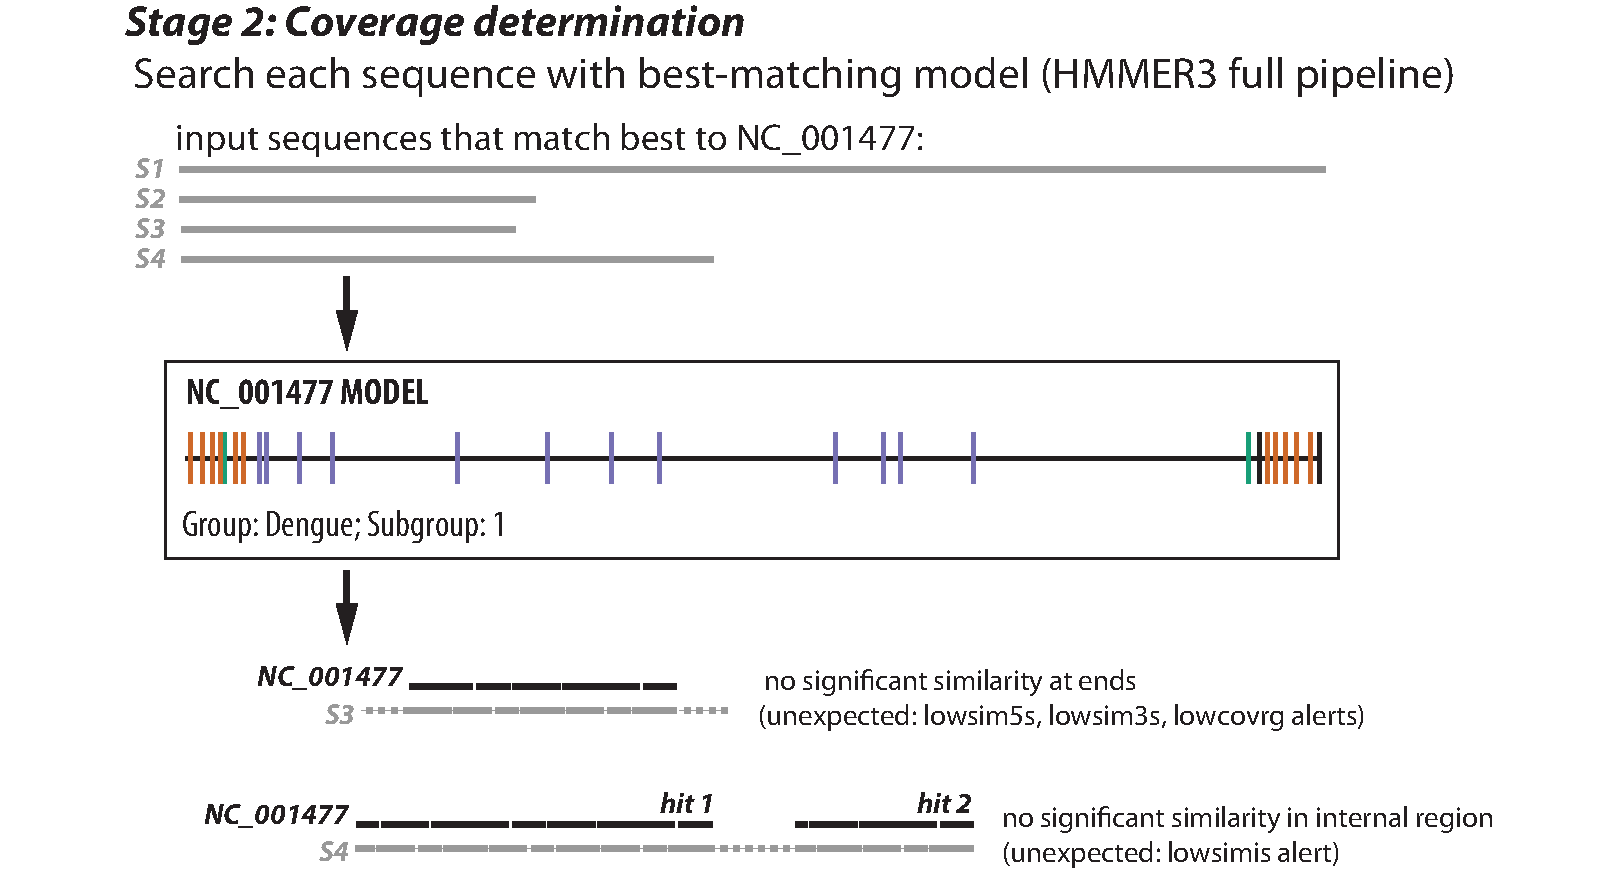
\includegraphics[width=10.5in]{figs/v-annotate-stage2-2}
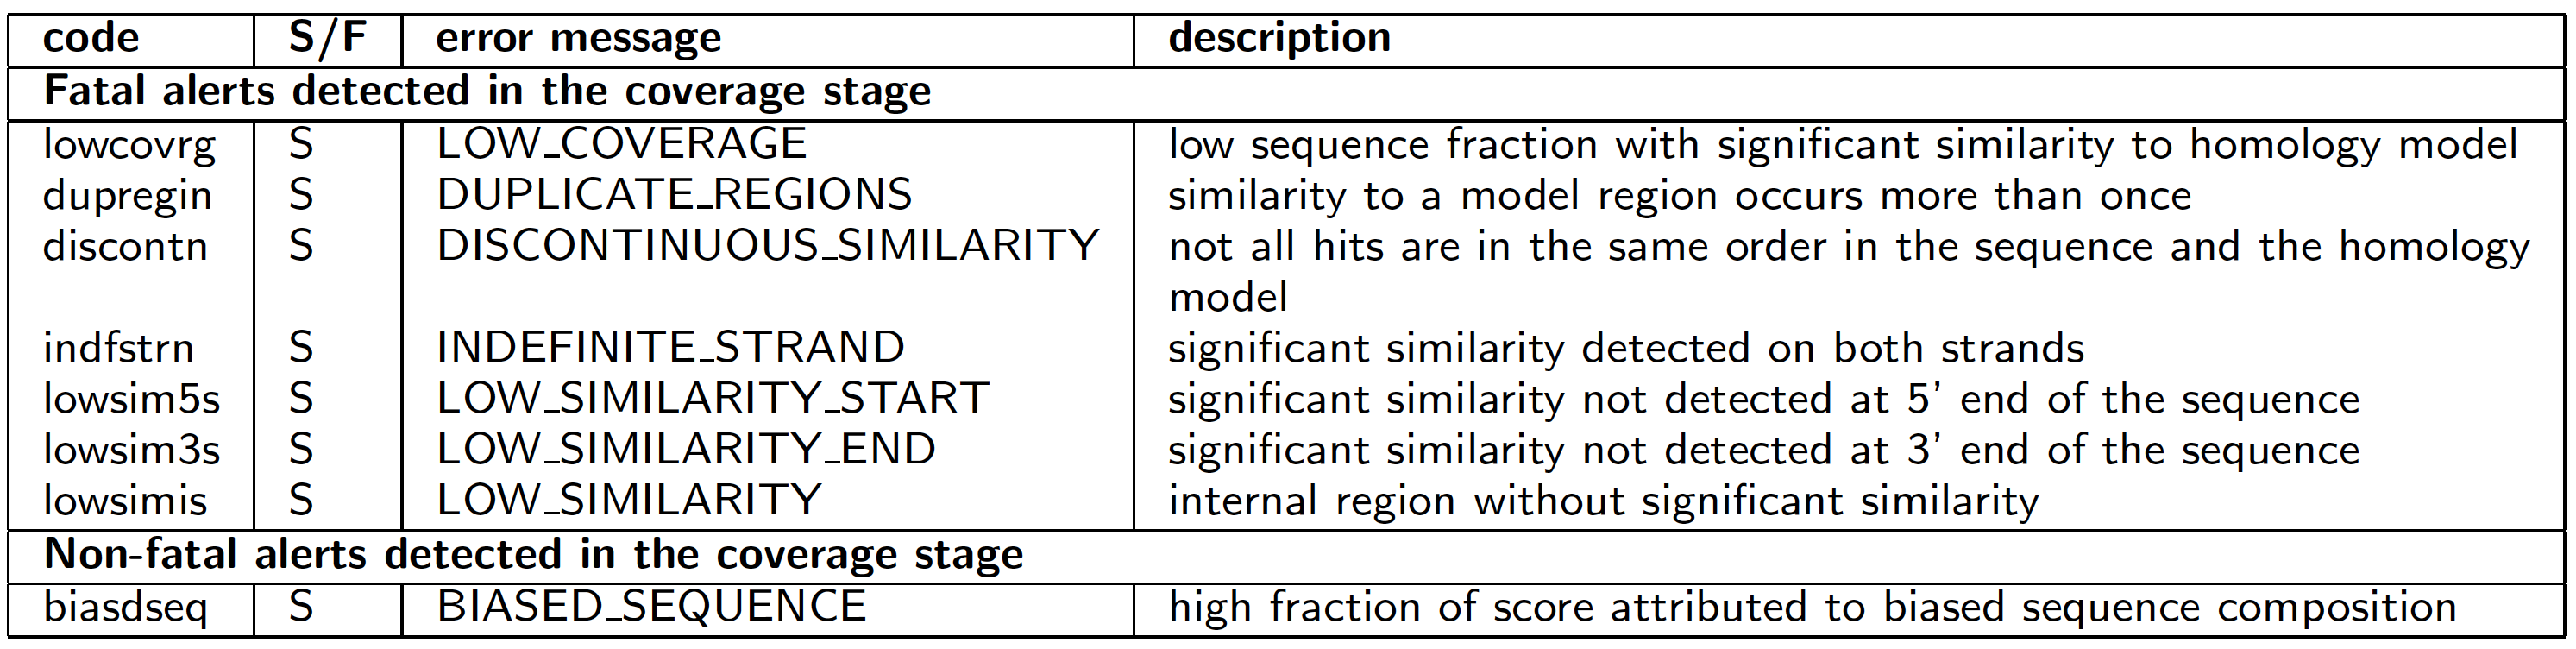
\includegraphics[width=10in]{figs/ss-coverage-alert-list}
\end{center}

\vfill
\end{slide}
%%%%%%%%%%%%%%%%%%%%%%%%%%%%%%%%%%%%%%%%%%%%%%%%%%%%%%%%%%%%%%%%%%%%%%
\begin{slide}
\begin{center}

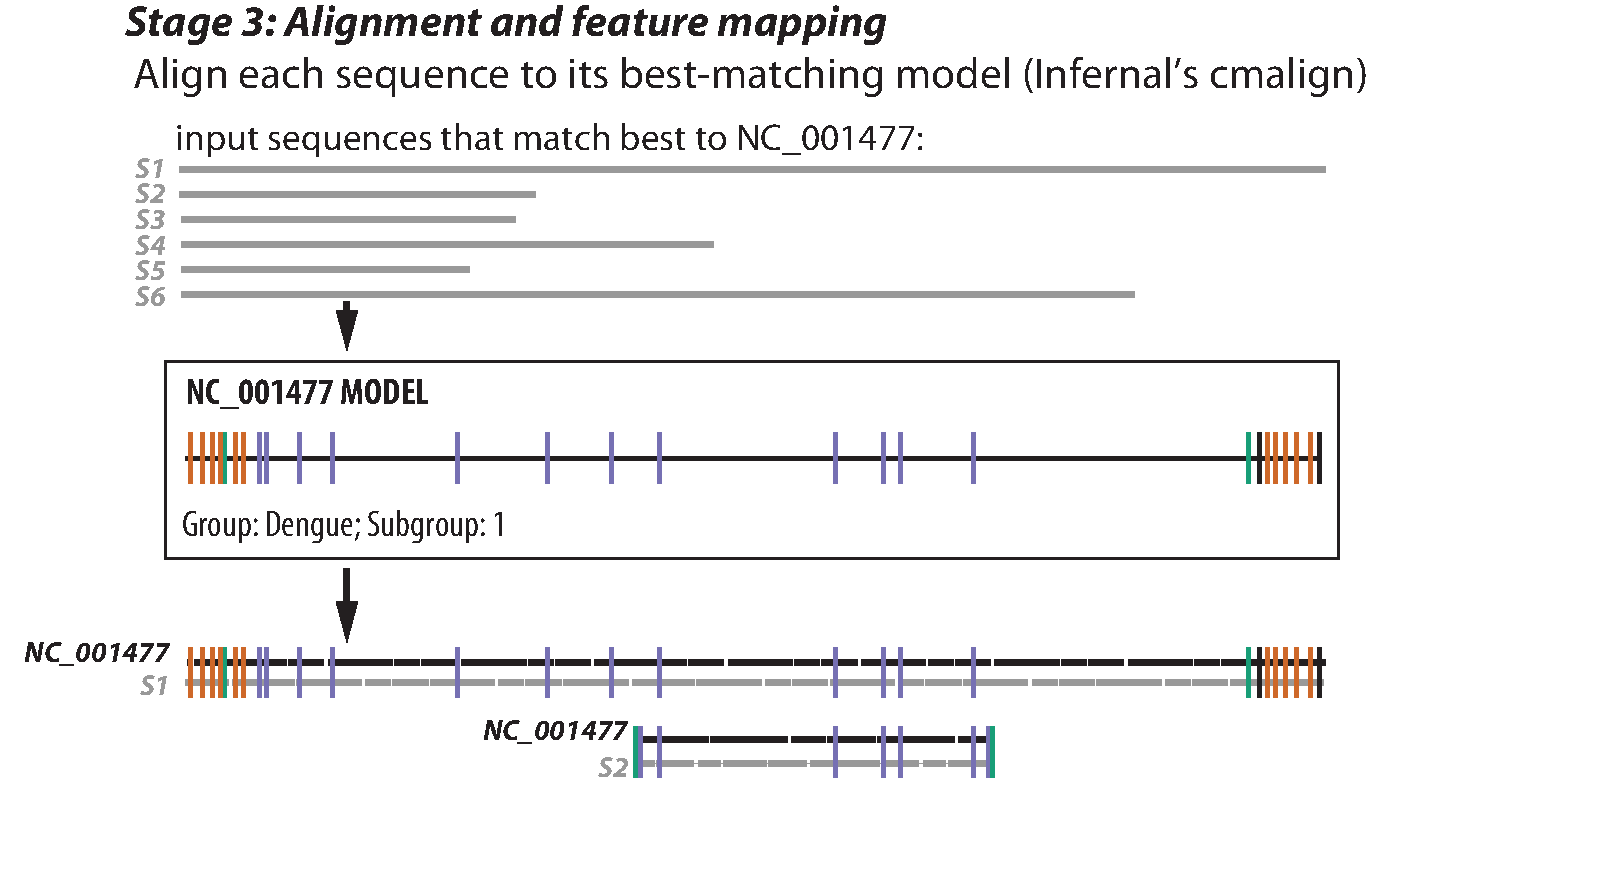
\includegraphics[width=10.5in]{figs/v-annotate-stage3-1}
\end{center}

\vfill
\end{slide}
%%%%%%%%%%%%%%%%%%%%%%%%%%%%%%%%%%%%%%%%%%%%%%%%%%%%%%%%%%%%%%%%%%%%%%
\begin{slide}
\begin{center}

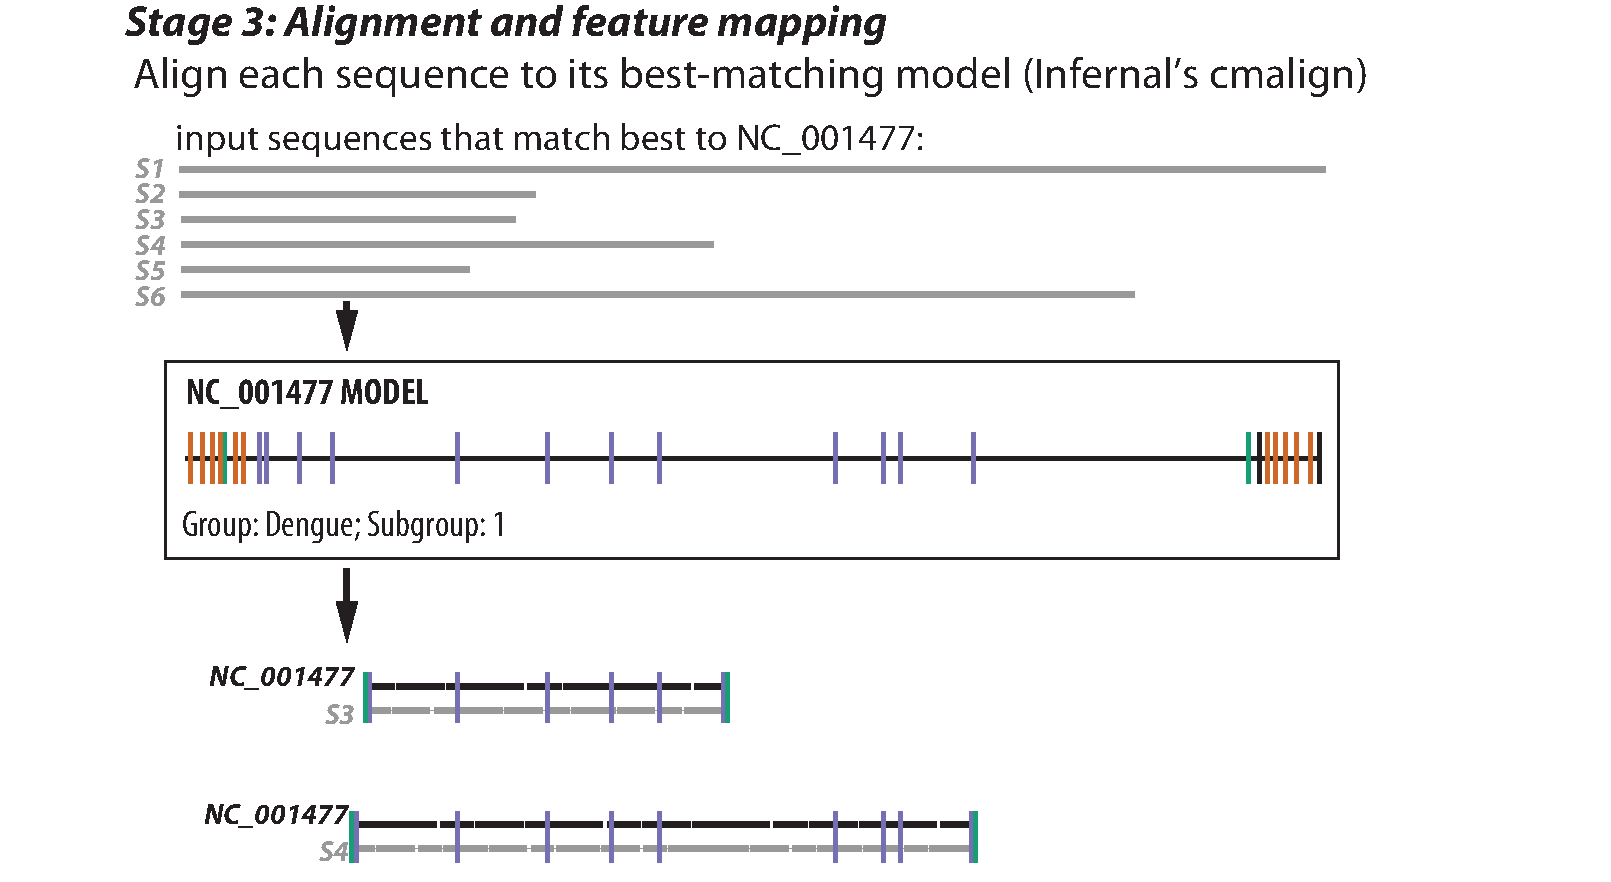
\includegraphics[width=10.5in]{figs/v-annotate-stage3-2}
\end{center}

\vfill
\end{slide}
%%%%%%%%%%%%%%%%%%%%%%%%%%%%%%%%%%%%%%%%%%%%%%%%%%%%%%%%%%%%%%%%%%%%%%
\begin{slide}
\begin{center}

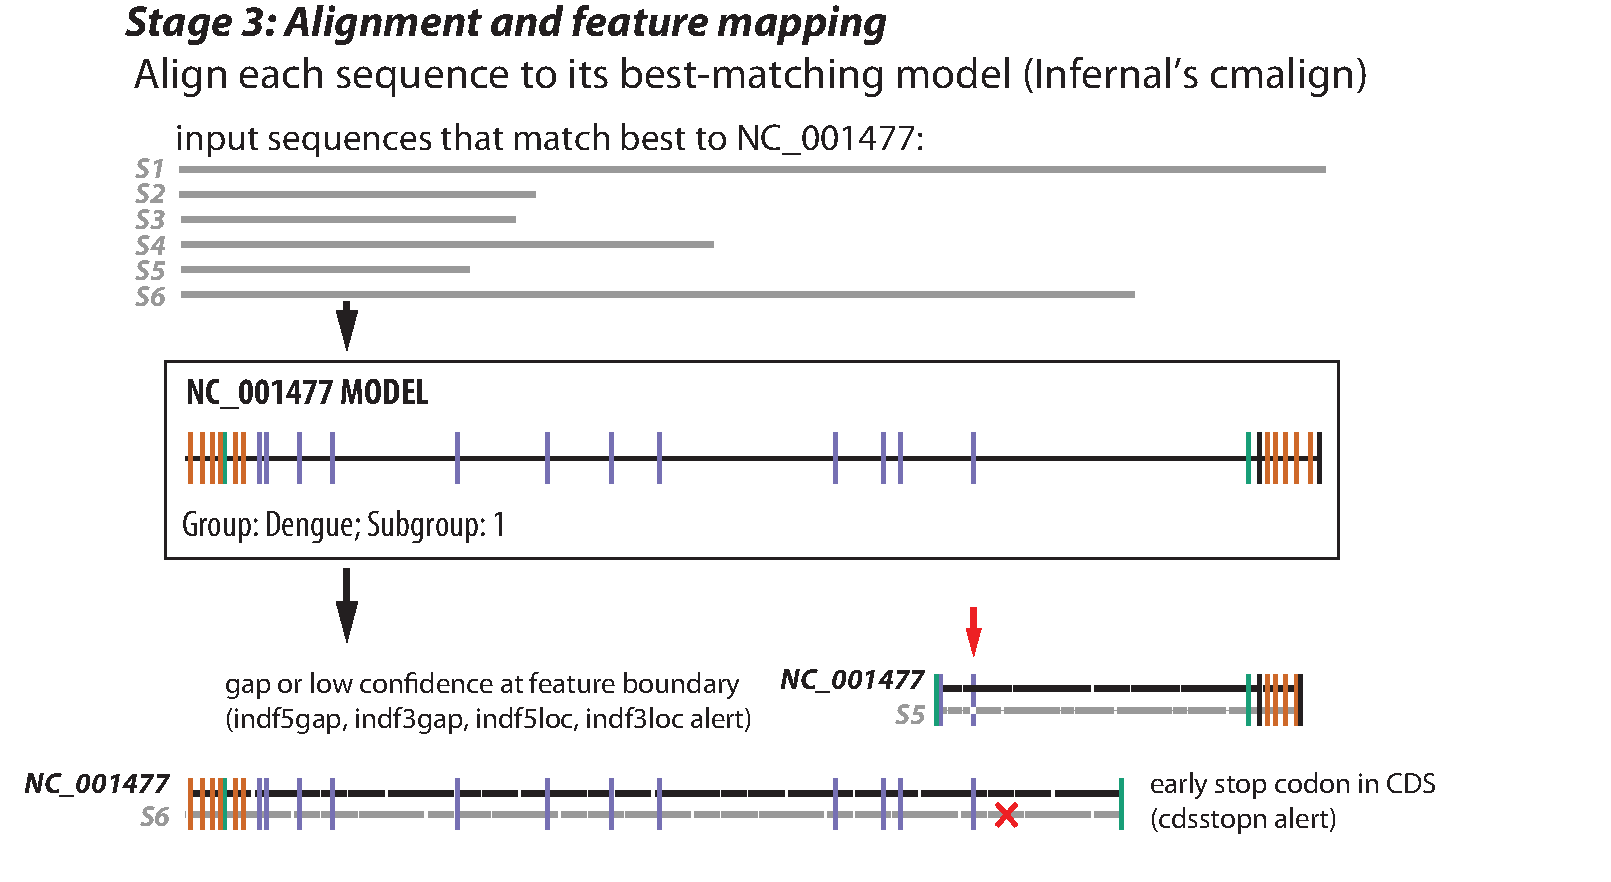
\includegraphics[width=10.5in]{figs/v-annotate-stage3-3}
\end{center}

\vfill
\end{slide}
%%%%%%%%%%%%%%%%%%%%%%%%%%%%%%%%%%%%%%%%%%%%%%%%%%%%%%%%%%%%%%%%%%%%%%
\begin{slide}
\begin{center}

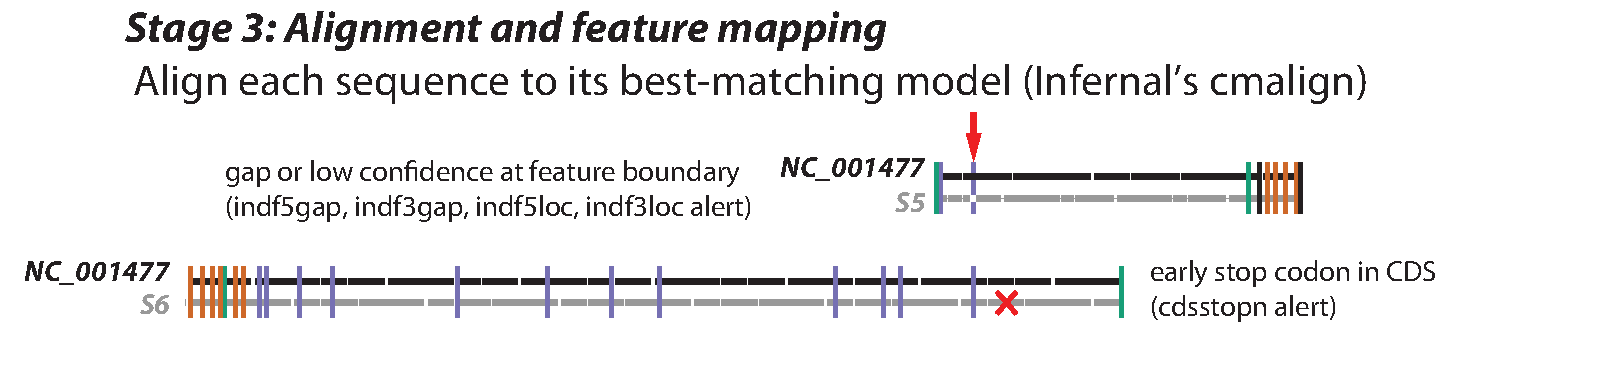
\includegraphics[width=10.5in]{figs/v-annotate-stage3-4}
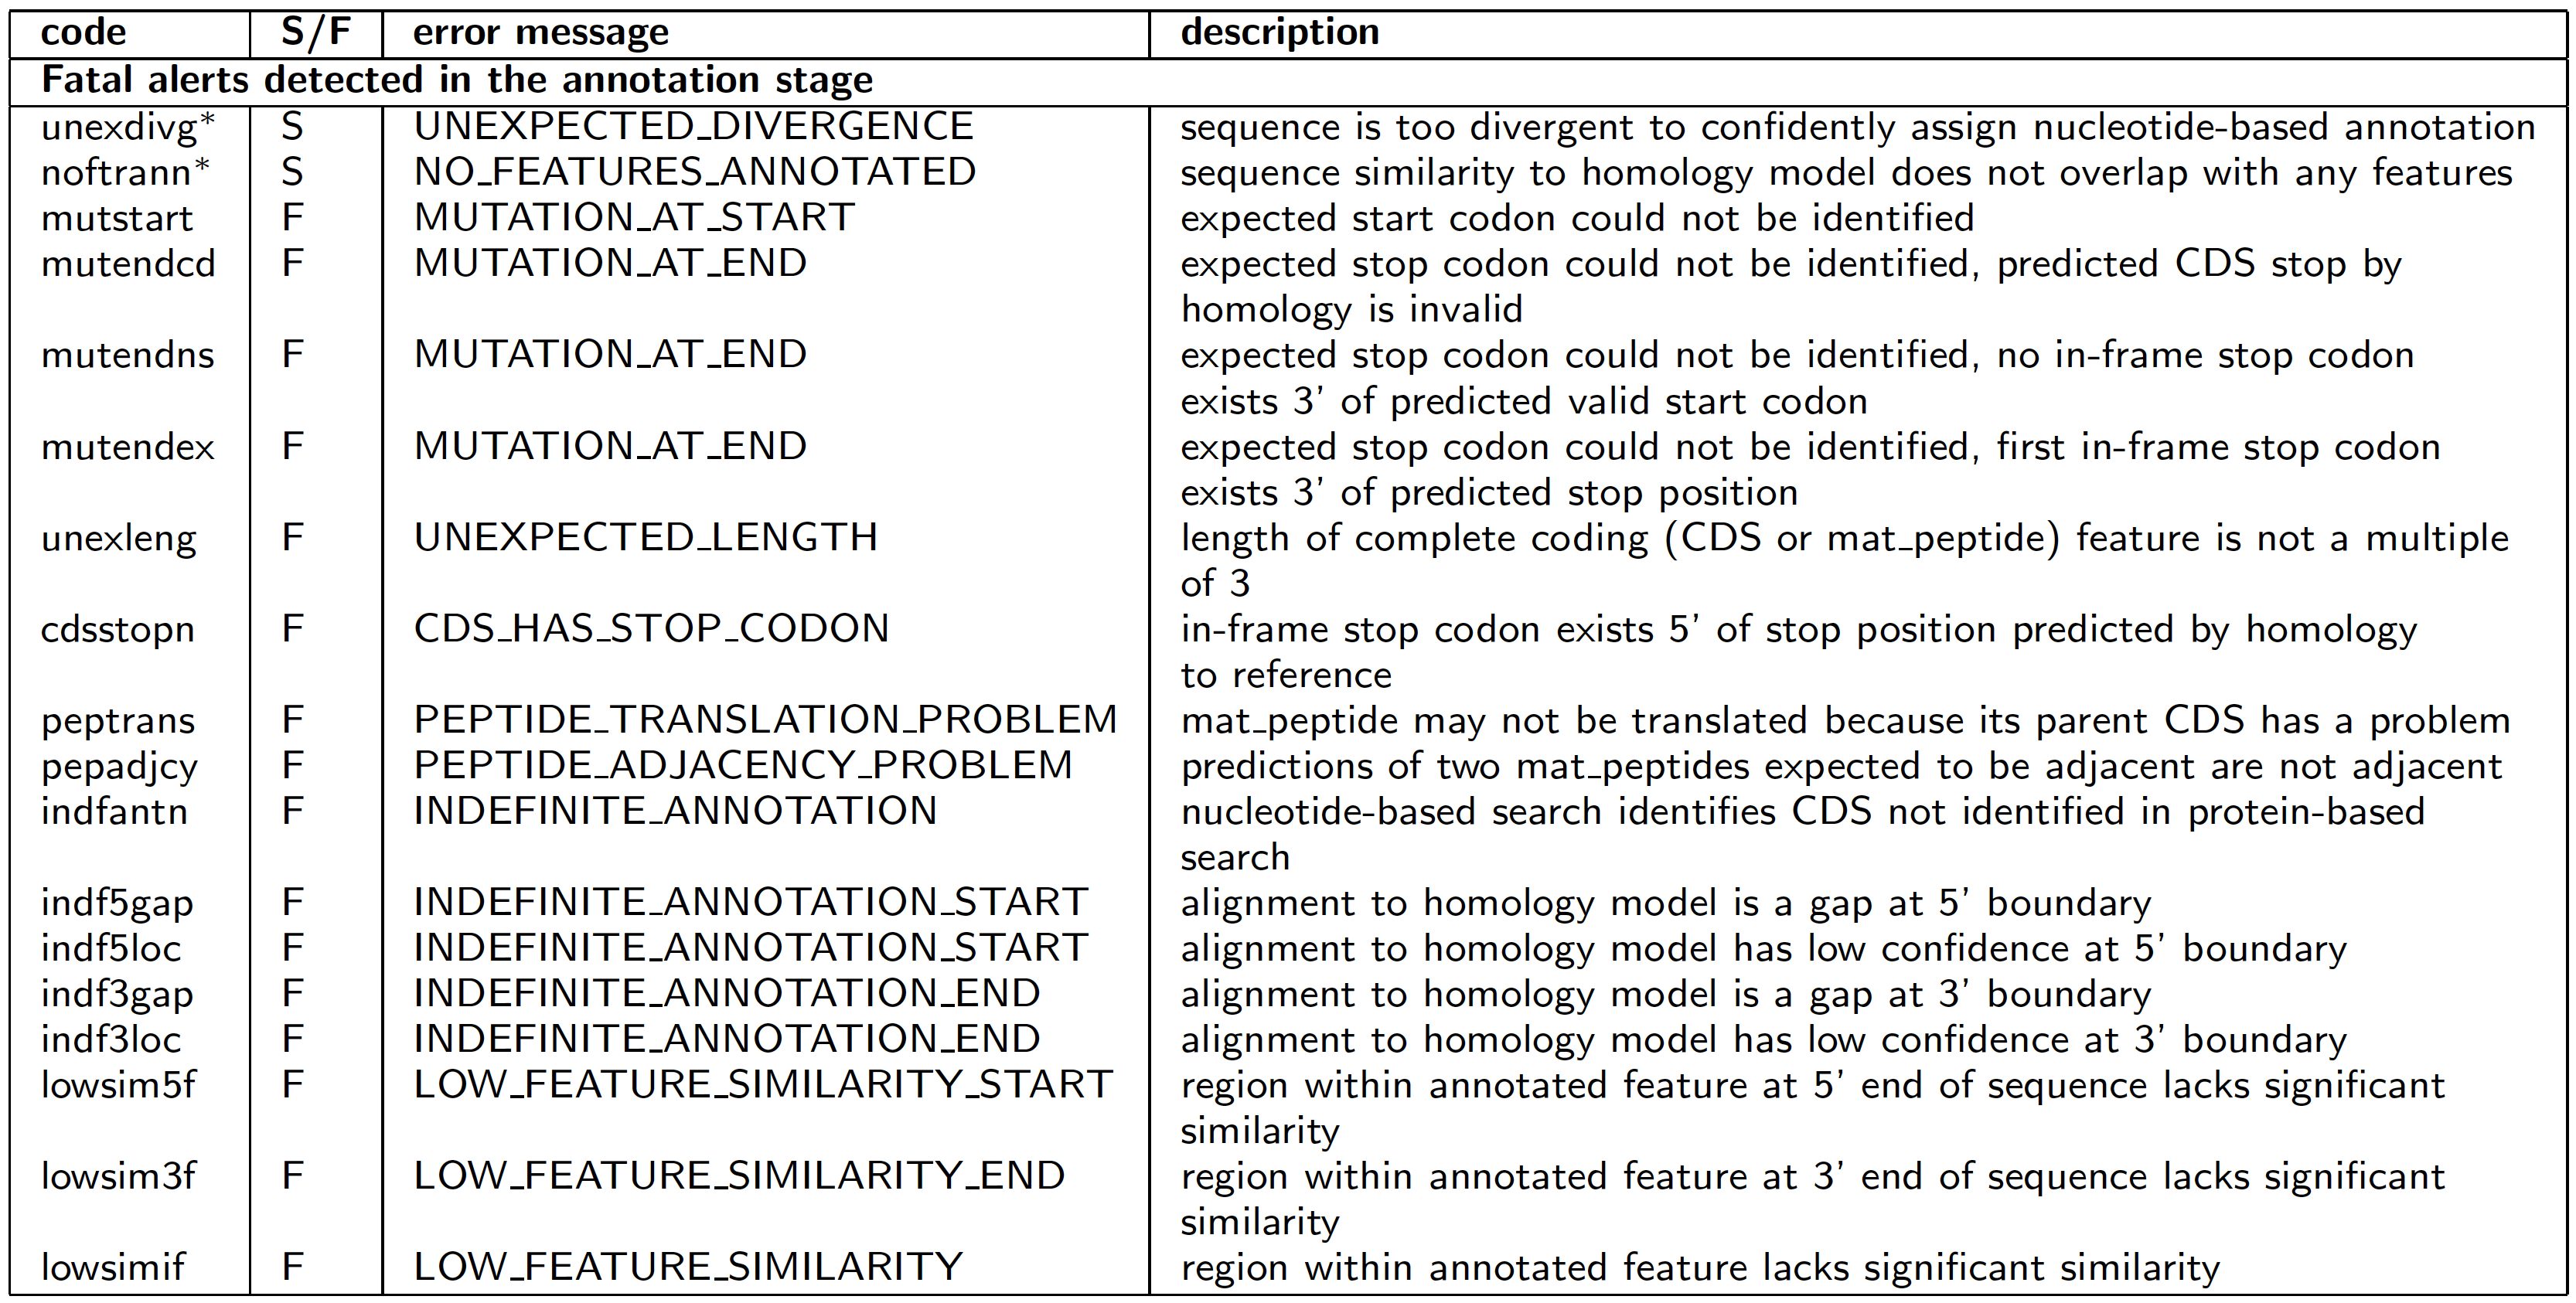
\includegraphics[width=10.5in]{figs/ss-alignment-alert-list}

\end{center}
\vfill
\end{slide}
%%%%%%%%%%%%%%%%%%%%%%%%%%%%%%%%%%%%%%%%%%%%%%%%%%%%%%%%%%%%%%%%%%%%%%
\begin{slide}
\begin{center}

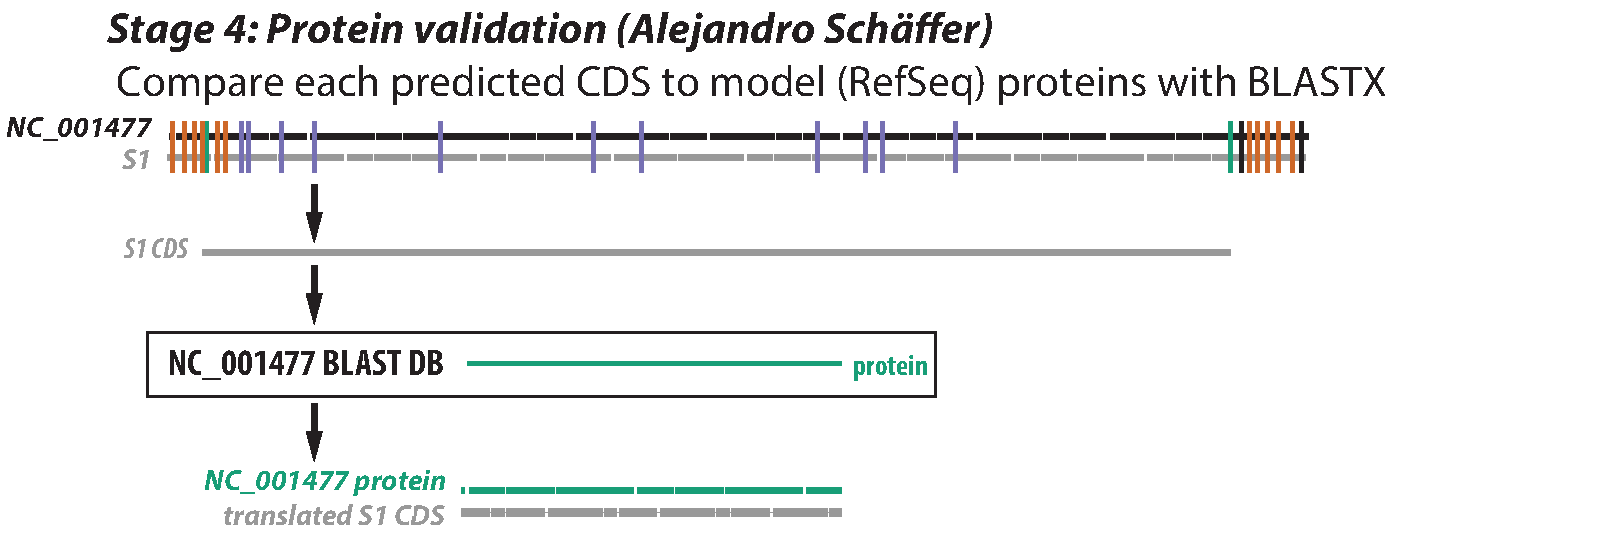
\includegraphics[width=10.5in]{figs/v-annotate-stage4-1}

\end{center}
\vfill
\end{slide}
%%%%%%%%%%%%%%%%%%%%%%%%%%%%%%%%%%%%%%%%%%%%%%%%%%%%%%%%%%%%%%%%%%%%%%
\begin{slide}
\begin{center}

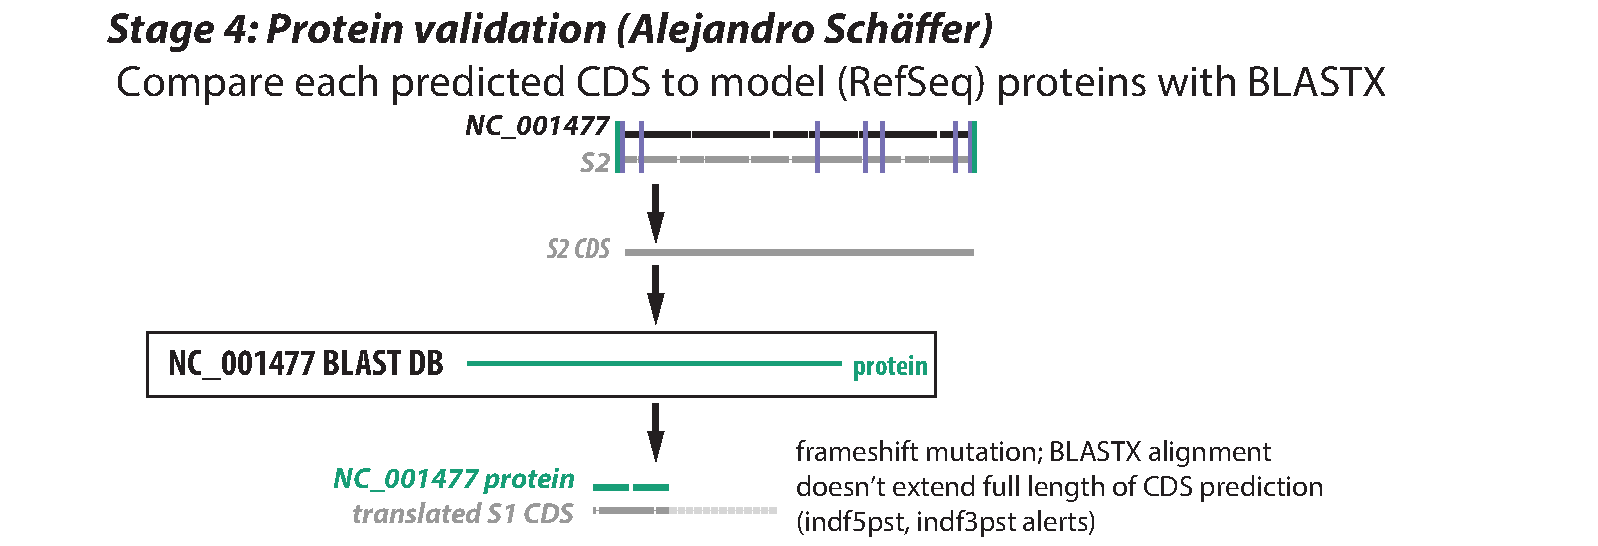
\includegraphics[width=10.5in]{figs/v-annotate-stage4-2}
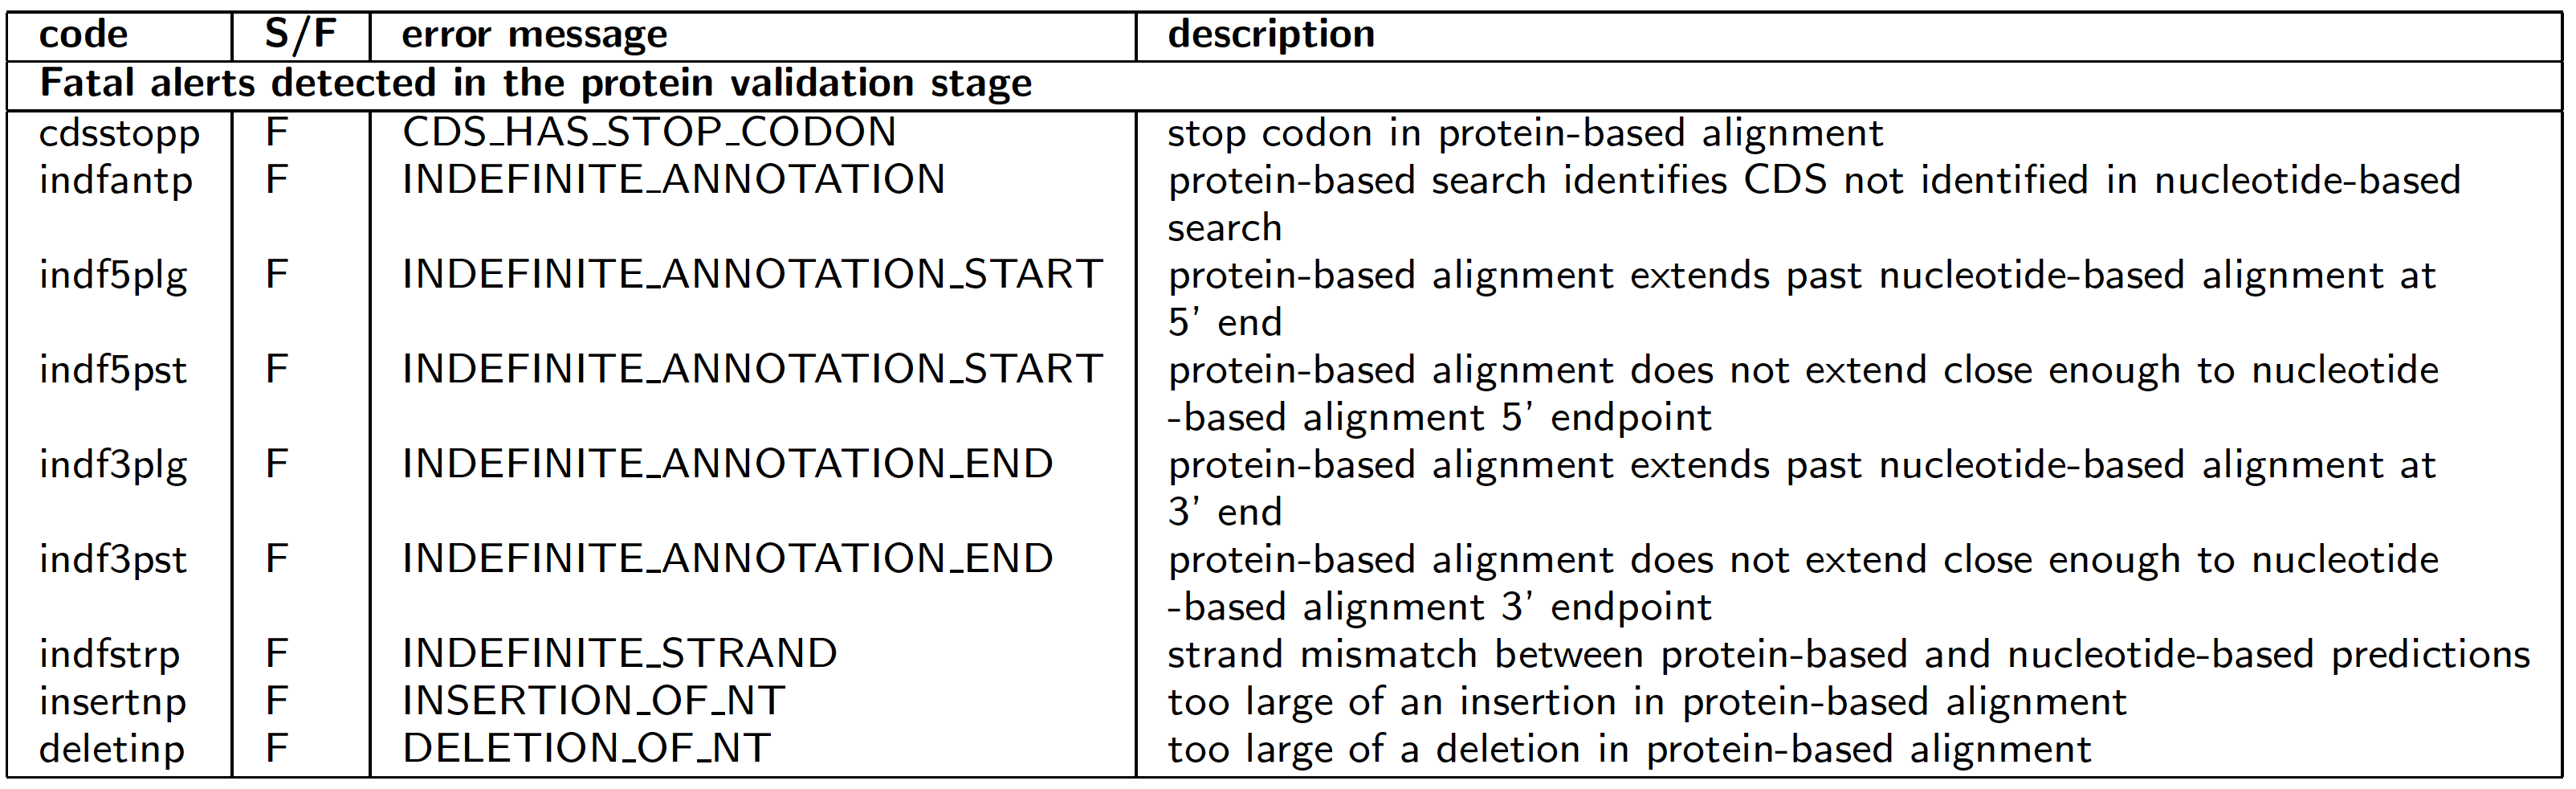
\includegraphics[width=10.5in]{figs/ss-protein-alert-list}

\end{center}
\vfill
\end{slide}
%%%%%%%%%%%%%%%%%%%%%%%%%%%%%%%%%%%%%%%%%%%%%%%%%%%%%%%%%%%%%%%%%%%%%%
\begin{slide}


\includegraphics[width=7in]{figs/blank-slide}
  
\vfill
\end{slide}
%%%%%%%%%%%%%%%%%%%%%%%%%%%%%%%%%%%%%%%%%%%%%%%%%%%%%%%%%%%%%%%%%%%%%%
\begin{slide}
\begin{center}
\includegraphics[width=10.5in]{figs/vadr-paper-title}
\end{center}

\small
\begin{itemize}
\item compared VADR to VAPiD and VIGOR programs on Norovirus and
  Dengue virus
\item VADR caught all the problems detected by VAPiD and VIGOR plus
  additional problems
\item 2809 of 3143 Norovirus sequences (89\%) tested with VADR passed (could foosh)
\item 1602 of 1702 Dengue sequences (94\%) tested with VADR passed
  (could foosh)
\end{itemize}  
  
\vfill
\end{slide}
%%%%%%%%%%%%%%%%%%%%%%%%%%%%%%%%%%%%%%%%%%%%%%%%%%%%%%%%%%%%%%%%%%%%%%
\begin{slide}
\begin{center}
\textbf{Limitations}
\end{center}

\small
\begin{itemize}
\item nucleotide space, not protein space
\item model (RefSeq) must be 'representative'
  \begin{itemize}
    \item divergent sequences, regions, introns, gene order are problematic
  \end{itemize}
\end{itemize}

\vfill
\end{slide}

%%%%%%%%%%%%%%%%%%%%%%%%%%%%%%%%%%%%%%%%%%%%%%%%%%%%%%%%%%%%%%%%%%%%%%
\begin{slide}
\begin{center}
\textbf{Limitations}
\end{center}

\small
\begin{itemize}
\item nucleotide space, not protein space
\item model (RefSeq) must be 'representative'
  \begin{itemize}
    \item divergent sequences, regions, introns, gene order are problematic
  \end{itemize}
\item current length limit of model is about 20Kb due to CM alignment memory
  requirements
\item slow
  \begin{itemize}
  \item Norovirus complete: 30 seconds/sequence (8X/6X slower than
    VAPiD/VIGOR)
  \item Dengue complete: 90 seconds/sequence (20X slower than VAPiD)
  \item Norovirus partial: 1.5 seconds/sequence (1.5X slower than VIGOR)
  \item Dengue partial: 9 seconds/sequence
  \end{itemize}
\end{itemize}

\vfill
\end{slide}
%%%%%%%%%%%%%%%%%%%%%%%%%%%%%%%%%%%%%%%%%%%%%%%%%%%%%%%%%%%%%%%%%%%%%%
\begin{slide}
\begin{center}
\textbf{Limitations}
\end{center}

\small
\begin{itemize}
\item nucleotide space, not protein space
\item model (RefSeq) must be 'representative'
  \begin{itemize}
    \item divergent sequences, regions, introns, gene order are problematic
  \end{itemize}
\item current length limit of model is about 20Kb due to CM alignment memory
  requirements
\item slow
  \begin{itemize}
  \item Norovirus complete: 30 seconds/sequence (8X/6X slower than
    VAPiD/VIGOR)
    % 1.5K NC
  \item Dengue complete: 90 seconds/sequence (20X slower than VAPiD)
    % 4.5K DC
  \item Norovirus partial: 1.5 seconds/sequence (1.5X slower than VIGOR)
    % 32K NP
  \item Dengue partial: 9 seconds/sequence
    % 21K DP
    % Noro:   1.5*30+32*1.5=93K seconds = 25 CPU hours
    % Dengue: 4.5*90+21*9= 594K seconds = 165 CPU hours
    % 190 hours / 8 cores = 24 hours on
  \end{itemize}
\item 190 CPU hours for all Norovirus and Dengue seqs (1 day on
8 core machine)
\end{itemize}

\vfill
\end{slide}
%%%%%%%%%%%%%%%%%%%%%%%%%%%%%%%%%%%%%%%%%%%%%%%%%%%%%%%%%%%%%%%%%%%%%%%
%%%%%%%%%%%%%%%%%%%%%%%%%%%%%%%%%%%%%%%%%%%%%%%%%%%%%%%%%%%%%%%%%%%%%%
\begin{slide}
\begin{center}
\textbf{VADR was designed to be flexible}
\end{center}

\small
\begin{itemize}
\item Any conserved sequence region $<$ 20Kb can be modeled 
\item VADR models are more powerful as profiles built from \textcolor{red}{\emph{alignments}} (RefAlign?)
\item Currently in testing for COX1: 
  \begin{itemize}
  \item Started with 9000 vetted COX1 protein sequences (Susan Schafer)
  \item Split based on taxonomy and aligned with MUSCLE
  \item Derived 43 \textcolor{red}{\emph{alignment-based}} models (e.g. \emph{Porifera}, \emph{Amphibia}) covering 5 genetic codes
  \item Classification stage compares against 43 models
  \item Protein validation stage compares against 9000 proteins
  \end{itemize}
%\item Goal: extend to other viruses and marker genes; building reference
%  sets and alignments is limiting
\end{itemize}

\vfill
\end{slide}
%%%%%%%%%%%%%%%%%%%%%%%%%%%%%%%%%%%%%%%%%%%%%%%%%%%%%%%%%%%%%%%%%%%%%%%%%
\begin{slide}
\begin{center}
\textbf{Future directions}
\end{center}

\small
\begin{itemize}
\item alignment-based models for viruses (testing with HCV)
\item profile-based protein validation to replace BLASTX
%\item allow scanning of large sequences (e.g. genomes)
\item extend to more viruses and genes, including ribosomal RNAs and possibly ITS
  sequences 
\end{itemize}

\vfill
\end{slide}
%%%%%%%%%%%%%%%%%%%%%%%%%%%%%%%%%%%%%%%%%%%%%%%%%%%%%%%%%%%%%%%%%%%%%%%%%
\begin{slide}

\large
\begin{center}
\large{\textbf{Acknowledgements}} \\

\normalsize
\vspace{0.75in}

\small
\begin{tabular}{l|l|l}
%                  & \\ \hline
%                  & \\
\textbf{NCBI - viral annotation} & \textbf{NCBI - leadership} &  \textbf{HMMER} \\
Alejandro Sch\"{a}ffer           & David Landsman             & Sean Eddy \\
Rodney Brister                   & Kim Pruitt                 & Travis Wheeler \\
Ilene Mizrachi                   & Jim Ostell                 & \\
Eneida Hatcher                   & David Lipman               & \\
Linda Yankie                     &                            & \\
Vincent Calhoun                  & \textbf{NLM - leadership}  & \\
Alex Kotliarov                   & Patti Brennan              & \\
Susan Schafer                    & Jerry Sheehan              & \\
Lara Shonkwiler                  & & \\
Sophia Hu                        & & \\
\end{tabular}


\includegraphics[width=2.5in]{figs/NIH_NLM_ABRV_2C_4-white}

\includegraphics[width=2.5in]{figs/ncbi-logo}

\end{center}

\vfill
\end{slide}


\begin{slide}
\begin{center}
\textbf{VADR results on all Norovirus and Dengue sequences}


%\scriptsize
%\begin{tabular}{l|r|r|r|r|r|r}
%                        &         & min    & max      &         &         & \textcolor{red}{fraction} \\
% dataset                & \# seqs & length & length   & \# pass & \# fail & \textcolor{red}{pass} \\ \hline
%Norovirus complete (NC) & 1,384    & 7380  & 7839     & 1,157    & 227     & \textcolor{red}{0.836} \\
%Dengue complete (DC)    & 4,580    & 10372 & 16254    & 4,171    & 409     & \textcolor{red}{0.911} \\
%& & & & & \\
%Norovirus partial (NP)  & 32,190   & 50    & 7376     & 29,488   & 2,702    & \textcolor{red}{0.916} \\
%Dengue partial (DP)     & 20,973   & 50    & 10370    & 17,276   & 3,697    & \textcolor{red}{0.824} \\
%\end{tabular}
\normalsize
\begin{tabular}{l|r|r|r|r}
                        &         &         &         & \textcolor{red}{fraction} \\
 dataset                & \# seqs & \# pass & \# fail & \textcolor{red}{pass} \\ \hline
Norovirus complete  & 1,384   & 1,157    & 227     & \textcolor{red}{0.836} \\
Dengue complete     & 4,580   & 4,171    & 409     & \textcolor{red}{0.911} \\
& & & & \\
Norovirus partial   & 32,190  & 29,488   & 2,702    & \textcolor{red}{0.916} \\
Dengue partial      & 20,973  & 17,276   & 3,697    & \textcolor{red}{0.824} \\
\end{tabular}

\end{center}
\vfill
\end{slide}
%%%%%%%%%%%%%%%%%%%%%%%%%%%%%%%%%%%%%%%%%%%%%%%%%%%%%%%%%%%%%%%%%%%%%%
\begin{slide}
\begin{center}
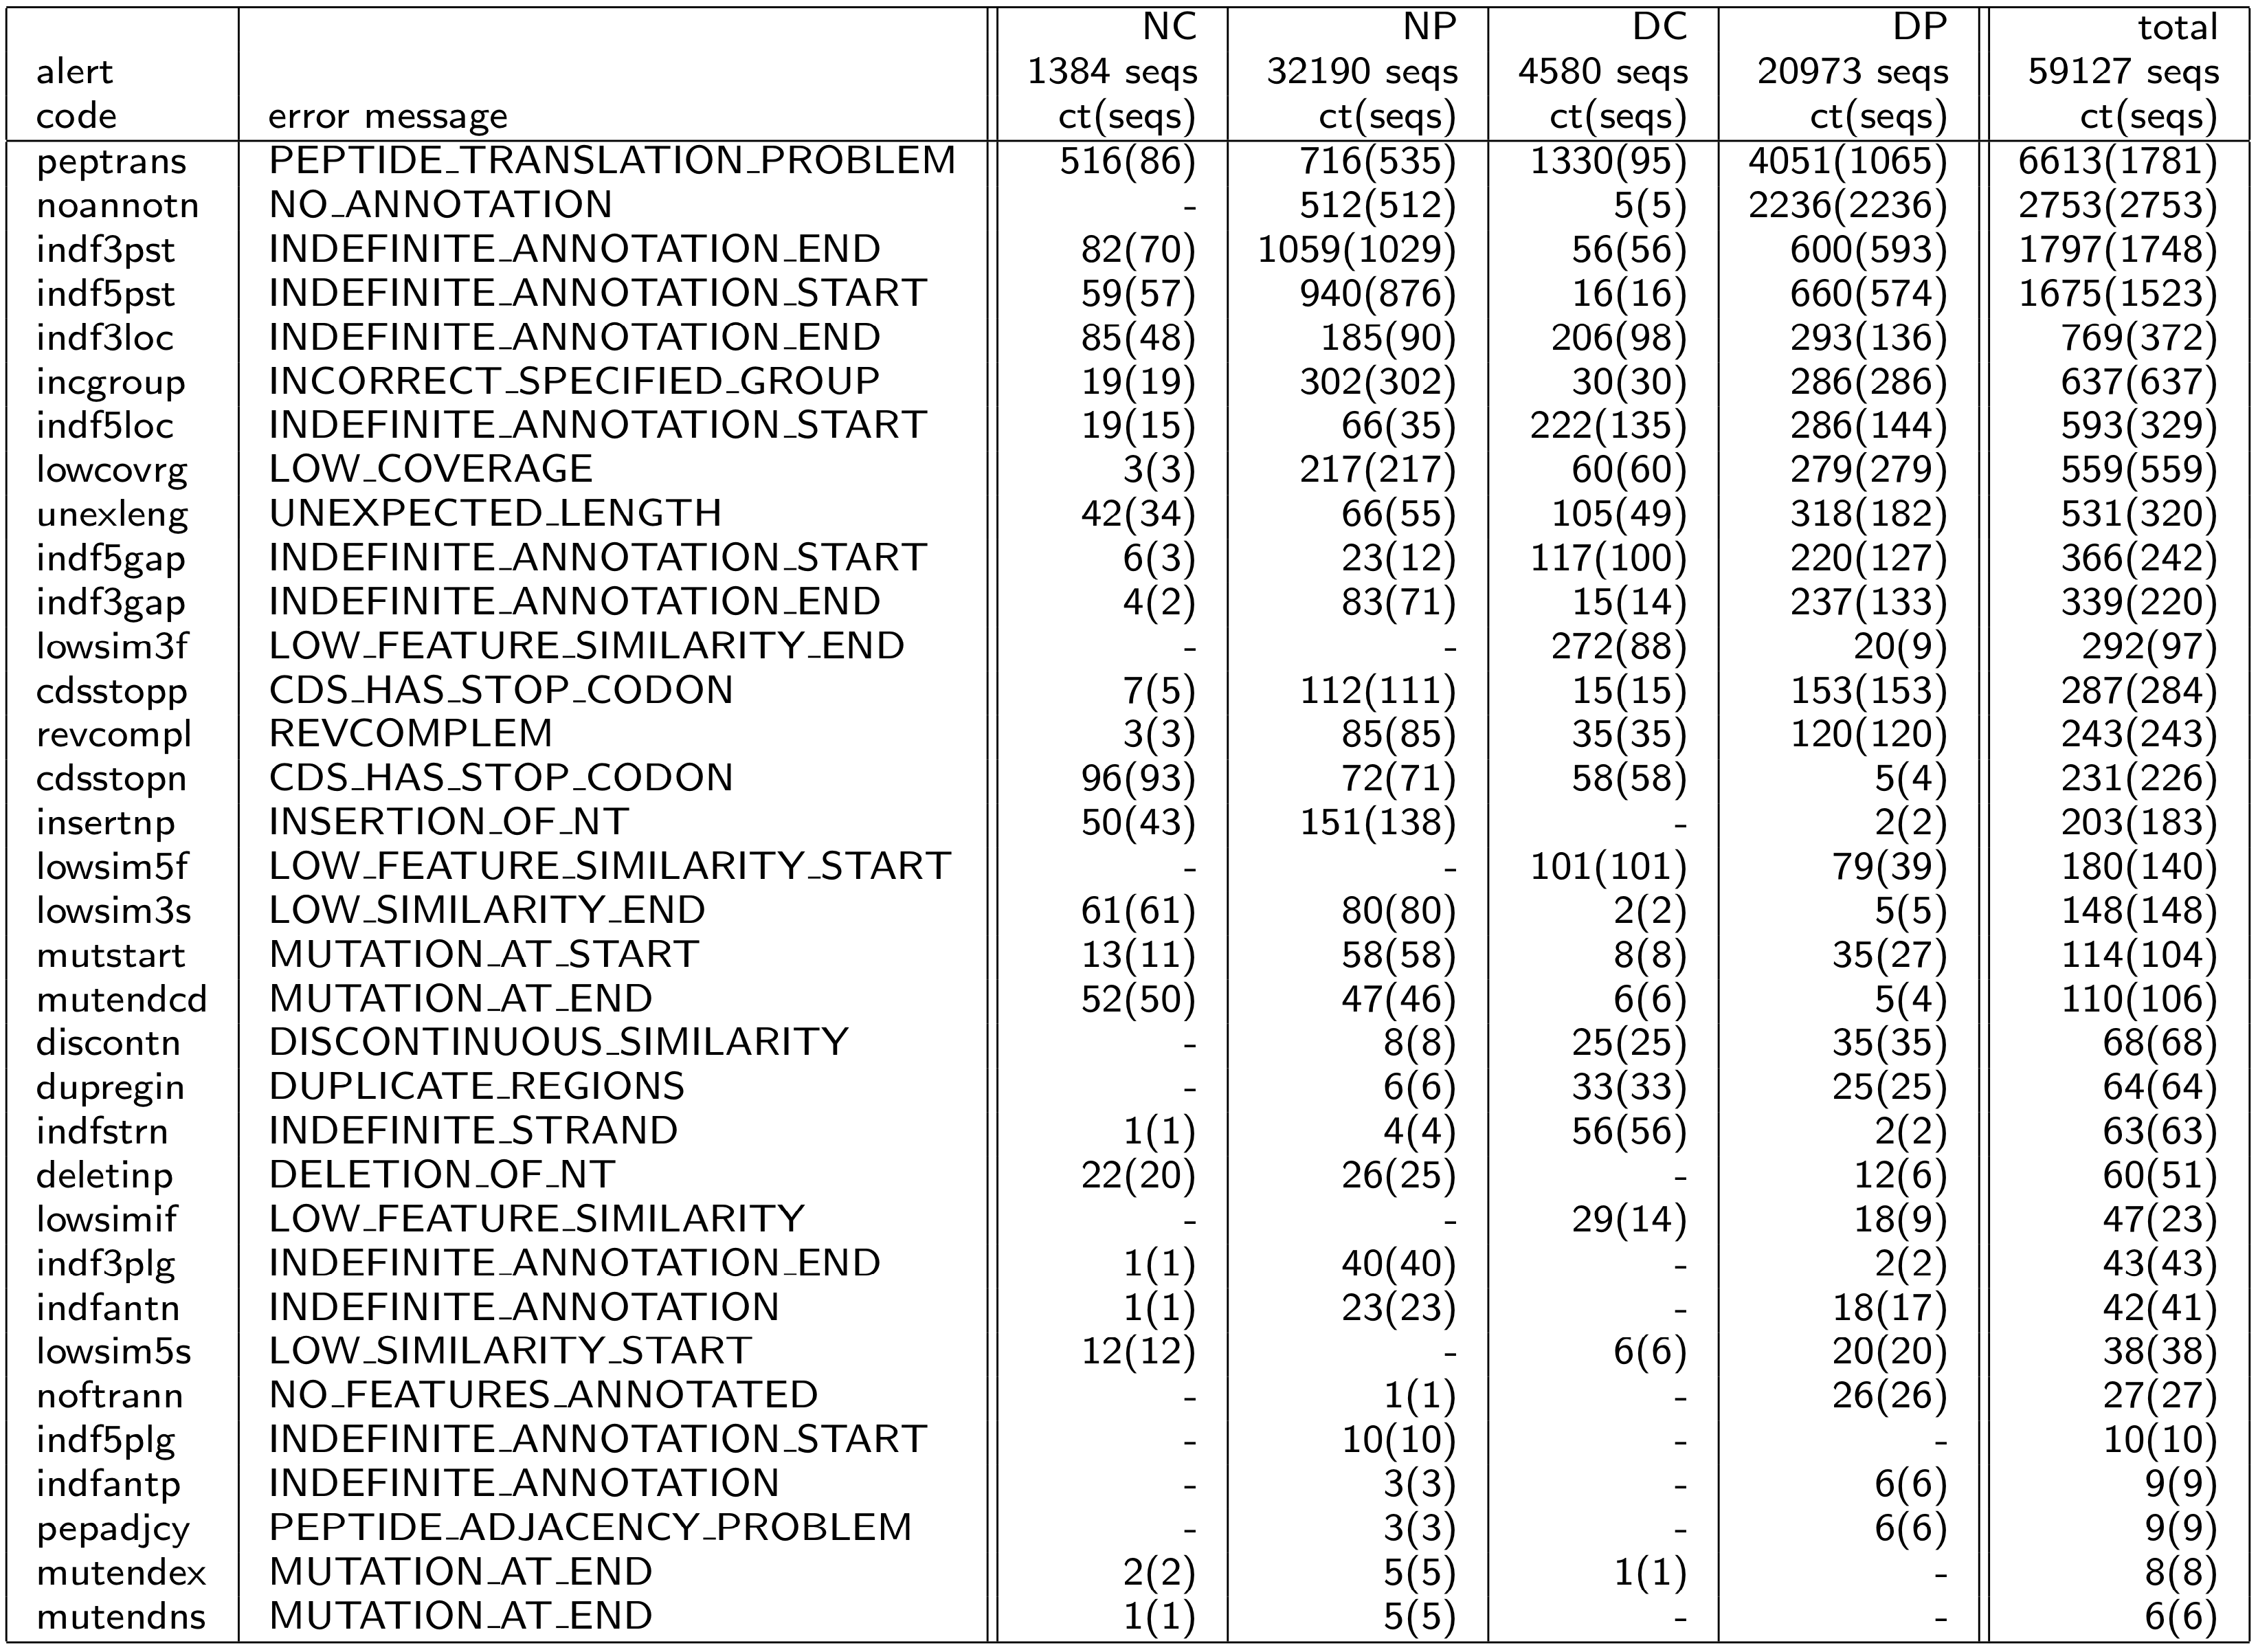
\includegraphics[width=10.5in]{figs/ss-alert-counts}
\end{center}

\vfill
\end{slide}
%%%%%%%%%%%%%%%%%%%%%%%%%%%%%%%%%%%%%%%%%%%%%%%%%%%%%%%%%%%%%%%%%%%%%%
\end{document}
%%%%%%%%%%%%%%%%%%%%%%%%%%%%%%%%%%%%%%%%%%%%%%%%%%%%%%%%%%%%%%%%%%%%%%
%%%%%%%%%%%%%%%%%%%%%%%%%%%%%%%%%%%%%%%%%%%%%%%%%%%%%%%%%%%%%%%%%%%%%%
%%%%%%%%%%%%%%%%%%%%%%%%%%%%%%%%%%%%%%%%%%%%%%%%%%%%%%%%%%%%%%%%%%%%%%
%%%%%%%%%%%%%%%%%%%%%%%%%%%%%%%%%%%%%%%%%%%%%%%%%%%%%%%%%%%%%%%%%%%%%%
%%%%%%%%%%%%%%%%%%%%%%%%%%%%%%%%%%%%%%%%%%%%%%%%%%%%%%%%%%%%%%%%%%%%%%
%%%%%%%%%%%%%%%%%%%%%%%%%%%%%%%%%%%%%%%%%%%%%%%%%%%%%%%%%%%%%%%%%%%%%%
\begin{slide}
\begin{center}
\textbf{Sequence submissions are handled by expert NCBI indexers}
\end{center}

\small
\begin{itemize}
\item Indexers check submissions for quality
\item Many submissions are of \emph{marker genes}, used to
  characterize environments (microbiome, soil), which are
  automatically analyzed by BLAST or specialized tools.
%\item Submissions with zero errors automatically enter database
%  (``foosh'')
%\item Submissions with errors can be corrected by submitter or are manually reviewed by an indexer
\end{itemize}

\medskip

\begin{center}
\begin{tabular}{l||r|r||r||l}
                                 &    2018  & total     &         &           \\
 marker gene/                    &  GenBank & GenBank   &  TLS\footnote{TLS: Targeted Locus Study, currently only 16S submissions with $>=$ 2500 seqs}      & analysis  \\
 sequence type                   &  \# seqs & \# seqs   & \# seqs & tool \\ \hline
& & & \\                    
%\textcolor{red}{16S rRNA}        & \textcolor{red}{333,121}  & \textcolor{red}{8,015,297} & \textcolor{red}{18,262,402} & \textcolor{red}{BLAST}\footnote{TLS submissions now processed with Ribosensor} \\
%16S rRNA                        & 333,121  & 8,015,297 & 18,262,402 & BLAST$^{*}$ \\
16S rRNA                        & 333,121  & 8,015,297 & 18,262,402 & BLAST \\
& & & \\                    
 23S rRNA                        & 74,287  &   275,014  & 2,140      & BLAST \\
& & & \\
 ITS1                            & 27,279  &   359,380  & 13,294     & BLAST \\
& & & \\                    
 ITS2                            & 24,144  &   184,515  &      0     & BLAST \\
& & & \\                    
 ITS1+ITS2                       & 26,734  &   445,721  & 25,725     & BLAST \\
& & & \\                    
 Influenza A                     & 74,868  &   665,464  &      0     & FLAN \\
\end{tabular}
\end{center}
\vfill
\tiny \flushleft{$\dagger$ TLS: Targeted Locus Study, currently only 16S submissions with $>=$ 2500 seqs, handled by Anji Johnston}
%\tiny \flushleft{$\ddagger$ TLS submissions now processed with ribosensor}
\end{slide}

\begin{slide}
\begin{center}

\includegraphics[width=10.5in]{figs/ss-vapid-title}
\end{center}

\small
\begin{itemize}
\item large reference database of nearly all complete genomes in
  GenBank
\item annotates each sequence based on best-match in reference
  database using blastn
\item designed for complete viral genomes
\item identifies early and absent stop codons and frameshift indels
\item simplifies submission by adding metadata expected by GenBank
\end{itemize}

\vfill
\end{slide}
%%%%%%%%%%%%%%%%%%%%%%%%%%%%%%%%%%%%%%%%%%%%%%%%%%%%%%%%%%%%%%%%%%%%%%
\begin{slide}
\begin{center}

\includegraphics[width=10.5in]{figs/ss-vigor-title}
\end{center}

\small
\begin{itemize}
\item determines most appropriate database (e.g. Norovirus)
  and annotates based on comparison of all proteins and mature
  peptides in that database
\item no Dengue database
\item identifies early and absent stop codons and frameshift indels
\end{itemize}

\vfill
\end{slide}
%%%%%%%%%%%%%%%%%%%%%%%%%%%%%%%%%%%%%%%%%%%%%%%%%%%%%%%%%%%%%%%%%%%%%%
\begin{slide}
\begin{center}
\textbf{Summary of VAPiD, VIGOR and VADR on 200 randomly chosen seqs}

\begin{tabular}{|l|r|r|r|}
\hline
         & VADR       & VAPiD     & VIGOR      \\
 dataset & pass/fail  & pass/fail & pass/fail  \\ \hline
       NC &  167/33 &  161/39 &   198/2 \\ 
       DC &  189/11 &   196/4 &       - \\ 
       NP &   191/9 &       - &   195/5 \\ 
       DP &  163/37 &       - &       - \\ 
\hline 
\end{tabular}
\end{center}

\vfill
\end{slide}
%%%%%%%%%%%%%%%%%%%%%%%%%%%%%%%%%%%%%%%%%%%%%%%%%%%%%%%%%%%%%%%%%%%%%%
\begin{slide}
\begin{center}
\textbf{Comparison of VAPiD and VADR}

\begin{tabular}{|l|r|r|r|r|}
\hline
          & Both       & Both       & VADR-pass  & VADR-fail  \\
 dataset  & pass       & fail       & VAPiD-fail & VAPiD-pass \\ \hline
       NC &        137 &          9 &         30 &     24 \\ 
       DC &        188 &          3 &          1 &      8 \\ 
\hline 
\end{tabular}

\end{center}

\vfill
\end{slide}
%%%%%%%%%%%%%%%%%%%%%%%%%%%%%%%%%%%%%%%%%%%%%%%%%%%%%%%%%%%%%%%%%%%%%%
\begin{slide}
\begin{center}
\textbf{Comparison of VAPiD and VADR}

\begin{tabular}{|l|r|r|r|r|}
\hline
          & Both       & Both       & VADR-pass  & VADR-fail  \\
 dataset  & pass       & fail       & VAPiD-fail & VAPiD-pass \\ \hline
       NC &        137 &          9 &         30 &     24 \\ 
       DC &        188 &          3 &          1 &      8 \\ 
\hline 
\end{tabular}

\small
\begin{itemize}
\item 12 that fail both:
  \begin{itemize}
  \item 9 have an internal stop or another
    CDS translation problem
  \item one has a start codon problem
  \item one is reverse complemented
  \item one fails because no reference is found
  \end{itemize}
\item 31 that fail only VAPiD are:
  \begin{itemize}
  \item 5' and/or 3' truncated in the first or final CDS
  \item 
    otherwise valid according to the VADR and VIGOR results
  \end{itemize}
\item \textcolor{red}{Conclusion: VADR finds all problems that VAPiD finds that should
  be caught.}
\end{itemize}
\end{center}

\vfill
\end{slide}
%%%%%%%%%%%%%%%%%%%%%%%%%%%%%%%%%%%%%%%%%%%%%%%%%%%%%%%%%%%%%%%%%%%%%%
\begin{slide}
\begin{center}
\textbf{Comparison of VIGOR and VADR}

\begin{tabular}{|l|r|r|r|r|}
\hline
         & Both       & Both       & VADR-pass  & VADR-fail  \\
 dataset & pass       & fail       & VIGOR-fail & VIGOR-pass \\ \hline
       NC &    167 &      2 &      0 &     31 \\ 
       NP &    191 &      5 &      0 &      4 \\ 
\hline 
\end{tabular}

\end{center}

\vfill
\end{slide}
%%%%%%%%%%%%%%%%%%%%%%%%%%%%%%%%%%%%%%%%%%%%%%%%%%%%%%%%%%%%%%%%%%%%%%
\begin{slide}
\begin{center}
\textbf{Comparison of VIGOR and VADR}

\begin{tabular}{|l|r|r|r|r|}
\hline
         & Both       & Both       & VADR-pass  & VADR-fail  \\
 dataset & pass       & fail       & VIGOR-fail & VIGOR-pass \\ \hline
      NC &        167 &          2 &          0 &     31 \\ 
      NP &        191 &          5 &          0 &      4 \\ 
\hline 
\end{tabular}

\small
\begin{itemize}
\item 7 that fail both:
  \begin{itemize}
  \item 3 have premature stops
  \item 2 are reverse complemented
  \item one has a frameshift 
  \item one fails because no similar reference is found
  \end{itemize}
\item \textcolor{red}{Conclusion: VADR finds all problems that VIGOR finds that should
  be caught.}
\end{itemize}
\end{center}

\vfill
\end{slide}

%%%%%%%%%%%%%%%%%%%%%%%%%%%%%%%%%%%%%%%%%%%%%%%%%%%%%%%%%%%%%%%%%%%%%%
\begin{slide}
\begin{center}
\textbf{35 sequences in NC, DC, and NP fail only VADR}

\small
\begin{itemize}
\item \textcolor{red}{These all have issues indexers want to manually review:}
\begin{itemize}
\item 16 sequences with early stops compared to closest RefSeqs %(\emph{cdsstopn})
\item 12 sequences for which BLASTX alignment does not extend close
  enough to alignment-based prediction %(\emph{indf5pst}, \emph{indf3pst})
\item 10 sequences with low similarity to RefSeq at 5' or 3' end of
  sequence or a feature %(lowsim5f, lowsim3f, or lowsim3s alerts)
\item 7 sequences where 5' or 3' boundary is a gap or not aligned with
  sufficient confidence (high enough posterior probability)
  %(indf5loc, indf5gap, or indf3loc alerts)
\item 5 sequences that are expected to be Norovirus but are really Sapovirus
  %(incgroup alerts)
\item 5 sequences with too large of an insertion/deletion in the
  BLASTX alignment %(insertnp or deletinp alerts)
\item 1 sequence not recognized by any of the \emph{Caliciviridae} or
  \emph{Flaviviridae} models (a Salivirus from \emph{Picornaviridae}
  family) %(noannotn alert)
\end{itemize}
\end{itemize}
\end{center}

\vfill
\end{slide}
%%%%%%%%%%%%%%%%%%%%%%%%%%%%%%%%%%%%%%%%%%%%%%%%%%%%%%%%%%%%%%%%%%%%%%
